\documentclass[editMode]{ufdissertation}\sloppy

%%%%%%%%%%%%%%%%%%%%%%%%%%%%%%%%%%%%%%%%%%%%%%%%%%%%%%%%%%%%%%%%%%%%%%%%%%%%%%%%
%%%                 User Package and Style File loading.
%%%%%%%%%%%%%%%%%%%%%%%%%%%%%%%%%%%%%%%%%%%%%%%%%%%%%%%%%%%%%%%%%%%%%%%%%%%%%%%%

%\usepackage{CustomMacros}%  This is a user macro/style file.

%\usepackage{tikz}%       tikz is used by almost everyone, but certainly by me for this.
%\usepackage{pgfplots}%   pgfplots is tikz but better.
%\usepackage{amsrefs}%   amsrefs contains the .bibtex style content for mathematician papers.
\usepackage{adjustbox}
\usepackage{graphicx}
\usepackage{amsmath}
\usepackage{listings}
\usepackage{color}

\newcommand\HI{{H\,\textsc{i}}} % neutral hydrogen
\newcommand\HII{{H\,\textsc{ii}}} % ionized hydrogen

\definecolor{mygray}{rgb}{0.4,0.4,0.4}
\definecolor{mygreen}{rgb}{0,0.8,0.6}
\definecolor{myorange}{rgb}{1.0,0.4,0}
\lstset{language=C++}
\lstset{
    basicstyle=\linespread{0.9}\ttfamily\color{black},
    commentstyle=\color{mygray},
    numbers=left,
    numbersep=5pt,
    numberstyle=\ttfamily\color{mygray},
    keywordstyle=\color{mygreen},
    showspaces=false,
    showstringspaces=false,
    stringstyle=\color{myorange},
    tabsize=4
}

%%%%%%%%%%%%%%%%%%%%%%%%%%%%%%%%%%%%%%%%%%%%%%%%%%%%%%%%%%%%%%%%%%%%%%%%%%%%%%%%
%%%                     User Configuration commands
%%%%%%%%%%%%%%%%%%%%%%%%%%%%%%%%%%%%%%%%%%%%%%%%%%%%%%%%%%%%%%%%%%%%%%%%%%%%%%%%

%% Uncomment the relevant line below if you have tables or figures.
\haveTablestrue%        Uncomment this if you have tables in your thesis.
\haveFigurestrue%       Uncomment this if you have figures in your thesis.
%\haveObjectstrue%       Uncomment this if you have Objects in your thesis. This is almost certainly not the case however.

% Standard journal abbreviations
% Mostly as used by ADS, with a few additions for journals where MNRAS does not
% follow normal IAU style.

\newcommand\aap{A\&A}                % Astronomy and Astrophysics
\let\astap=\aap                          % alternative shortcut
\newcommand\aapr{A\&ARv}             % Astronomy and Astrophysics Review (the)
\newcommand\aaps{A\&AS}              % Astronomy and Astrophysics Supplement Series
\newcommand\actaa{Acta Astron.}      % Acta Astronomica
\newcommand\afz{Afz}                 % Astrofizika
\newcommand\aj{AJ}                   % Astronomical Journal (the)
\newcommand\ao{Appl. Opt.}           % Applied Optics
\let\applopt=\ao                         % alternative shortcut
\newcommand\aplett{Astrophys.~Lett.} % Astrophysics Letters
\newcommand\apj{ApJ}                 % Astrophysical Journal
\newcommand\apjl{ApJ}                % Astrophysical Journal, Letters
\let\apjlett=\apjl                       % alternative shortcut
\newcommand\apjs{ApJS}               % Astrophysical Journal, Supplement
\let\apjsupp=\apjs                       % alternative shortcut
% The following journal does not appear to exist! Disabled.
%\newcommand\apspr{Astrophys.~Space~Phys.~Res.} % Astrophysics Space Physics Research
\newcommand\apss{Ap\&SS}             % Astrophysics and Space Science
\newcommand\araa{ARA\&A}             % Annual Review of Astronomy and Astrophysics
\newcommand\arep{Astron. Rep.}       % Astronomy Reports
\newcommand\aspc{ASP Conf. Ser.}     % ASP Conference Series
\newcommand\azh{Azh}                 % Astronomicheskii Zhurnal
\newcommand\baas{BAAS}               % Bulletin of the American Astronomical Society
\newcommand\bac{Bull. Astron. Inst. Czechoslovakia} % Bulletin of the Astronomical Institutes of Czechoslovakia 
\newcommand\bain{Bull. Astron. Inst. Netherlands} % Bulletin Astronomical Institute of the Netherlands
\newcommand\caa{Chinese Astron. Astrophys.} % Chinese Astronomy and Astrophysics
\newcommand\cjaa{Chinese J.~Astron. Astrophys.} % Chinese Journal of Astronomy and Astrophysics
\newcommand\fcp{Fundamentals Cosmic Phys.}  % Fundamentals of Cosmic Physics
\newcommand\gca{Geochimica Cosmochimica Acta}   % Geochimica Cosmochimica Acta
\newcommand\grl{Geophys. Res. Lett.} % Geophysics Research Letters
\newcommand\iaucirc{IAU~Circ.}       % IAU Cirulars
\newcommand\icarus{Icarus}           % Icarus
\newcommand\japa{J.~Astrophys. Astron.} % Journal of Astrophysics and Astronomy
\newcommand\jcap{J.~Cosmology Astropart. Phys.} % Journal of Cosmology and Astroparticle Physics
\newcommand\jcp{J.~Chem.~Phys.}      % Journal of Chemical Physics
\newcommand\jgr{J.~Geophys.~Res.}    % Journal of Geophysics Research
\newcommand\jqsrt{J.~Quant. Spectrosc. Radiative Transfer} % Journal of Quantitiative Spectroscopy and Radiative Transfer
\newcommand\jrasc{J.~R.~Astron. Soc. Canada} % Journal of the RAS of Canada
\newcommand\memras{Mem.~RAS}         % Memoirs of the RAS
\newcommand\memsai{Mem. Soc. Astron. Italiana} % Memoire della Societa Astronomica Italiana
\newcommand\mnassa{MNASSA}           % Monthly Notes of the Astronomical Society of Southern Africa
\newcommand\mnras{MNRAS}             % Monthly Notices of the Royal Astronomical Society
\newcommand\na{New~Astron.}          % New Astronomy
\newcommand\nar{New~Astron.~Rev.}    % New Astronomy Review
\newcommand\nat{Nature}              % Nature
\newcommand\nphysa{Nuclear Phys.~A}  % Nuclear Physics A
\newcommand\pra{Phys. Rev.~A}        % Physical Review A: General Physics
\newcommand\prb{Phys. Rev.~B}        % Physical Review B: Solid State
\newcommand\prc{Phys. Rev.~C}        % Physical Review C
\newcommand\prd{Phys. Rev.~D}        % Physical Review D
\newcommand\pre{Phys. Rev.~E}        % Physical Review E
\newcommand\prl{Phys. Rev.~Lett.}    % Physical Review Letters
\newcommand\pasa{Publ. Astron. Soc. Australia}  % Publications of the Astronomical Society of Australia
\newcommand\pasp{PASP}               % Publications of the Astronomical Society of the Pacific
\newcommand\pasj{PASJ}               % Publications of the Astronomical Society of Japan
\newcommand\physrep{Phys.~Rep.}      % Physics Reports
\newcommand\physscr{Phys.~Scr.}      % Physica Scripta
\newcommand\planss{Planet. Space~Sci.} % Planetary Space Science
\newcommand\procspie{Proc.~SPIE}     % Proceedings of the Society of Photo-Optical Instrumentation Engineers
\newcommand\rmxaa{Rev. Mex. Astron. Astrofis.} % Revista Mexicana de Astronomia y Astrofisica
\newcommand\qjras{QJRAS}             % Quarterly Journal of the RAS
\newcommand\sci{Science}             % Science
\newcommand\skytel{Sky \& Telesc.}   % Sky and Telescope
\newcommand\solphys{Sol.~Phys.}      % Solar Physics
\newcommand\sovast{Soviet~Ast.}      % Soviet Astronomy (aka Astronomy Reports)
\newcommand\ssr{Space Sci. Rev.}     % Space Science Reviews
\newcommand\zap{Z.~Astrophys.}       % Zeitschrift fuer Astrophysik

\newcommand{\red}[1]{{\textcolor{red}{#1}}}

%%%%%%%%%%%%%%%%%%%%%%%%%%%%%%%%%%%%%%%%%%%%%%%%%%%%%%%%%%%%%%%%%%%%%%%%%%%%%%%%
%%% Below are the commands to set the degree type, department, graduation time, and chair. 
%       Most of these are self explanatory. 
%       Note: The \chair command takes an optional argument for a cochair. 
%           So if John was your chair and Jacob was a cochair, you would use \chair[Jacob]{John}.
%           If John was your chair and you had no cochair, you can simply use \chair{John}.
%%%%%%%%%%%%%%%%%%%%%%%%%%%%%%%%%%%%%%%%%%%%%%%%%%%%%%%%%%%%%%%%%%%%%%%%%%%%%%%%

\title{Lyman-alpha Blobs in Cosmological Simulations}

\degreeType{Doctor of Philosophy}
\major{Astronomy}
\author{Benjamin Kimock}
\thesisType{Dissertation}
\degreeYear{2020}
\degreeMonth{May}
\chair{Desika Narayanan}


%%%%%%%%%%%%%%%%%%%%%%%%%%%%%%%%%%%%%%%%%%%%%%%%%%%%%%%%%%%%%%%%%%%%%%%%%%%%%%%%
%%% For each of the following, type in the name of the file that contains each section. 
%       They are assumed to be tex files, but if they aren't the command takes an optional argument for the extension.
%       So, you could load dedication.tex as your dedication file using \setDedicationFile{dedication}
%       You could load dedication.txt instead with \setDedicationFile[txt]{dedication}.
%       NOTE: For some compilers they may or may not add a .tex to the end of the file automatically.
%           If you get a "couldn't find dedication.tex.tex" type error, try the command with an empty optional argument,
%           e.g. \setDedicationFile[]{dedication}
%%%
%%%%%%%%%%%%%%%%%%%%%%%%%%%%%%%%%%%%%%%%%%%%%%%%%%%%%%%%%%%%%%%%%%%%%%%%%%%%%%%%

%%% These are REQUIRED sections; easiest to do via these commands.

\setDedicationFile{dedicationFile}%                 Dedication Page
\setAcknowledgementsFile{acknowledgementsFile}%     Acknowledgements Page
\setAbstractFile{abstractFile}%                     Abstract Page (This should only include the abstract itself)
\setReferenceFile{biblio}{mnras}%         References. First argument is your bibtex source file
%                                                       the second argument is your bibtex style file.
\setBiographicalFile{biographyFile}%                Biography file of the Author (you).

%%% These are NOT required, so only use them if you actually need/have them.

%\setAbbreviationsFile{abbreviations}%         Abbreviations Page
\setAppendixFile{appendix}%                    Appendix Content; hyperlinking might be weird.
%\multipleAppendixtrue%                         Uncomment this if you have more than one appendix,
%                                                   comment it if you have only one appendix.

%%%%%%%                     End of File Assignment
%%%%%%%%%%%%%%%%%%%%%%%%%%%%%%%%%%%%%%%%%%%%%%%%%%%%%%%%%%%%%%%%%%%%%%%%%%%%%%%%

\begin{document}

\chapter{Introduction and Opening Remarks}
\label{sec:intro}

Lyman-$\alpha$ "blobs" (LABs) are an enigmatic class of objects first discovered roughly $2$ decades ago \citep{Fynbo1999,Steidel2000}, and are characterized by copious Ly$\alpha$ luminosity, as well as their large spatial extent.
While there are no hard constraints on the definition of a blob, the majority of blobs have luminosities $L_{\rm{Ly}\alpha} > 10^{43}$ erg/s, and spatial extents that exceed $\sim50$ kpc in radius.
We will discuss this definition in more detail shortly.

Observing Ly$\alpha$ blobs is an interesting subject in itself, and since observational signatures have motivated a large fraction of this work we include some explanation of that issue.
The Ly$\alpha$ line's rest-frame wavelength is $\sim 1215.67 \AA$, and thus is mostly observed between $z=2$ and $z=5$, because within that range it is redshifted into the optical range where the atmosphere is transparent (see Table~\ref{table:labs}).

Ly$\alpha$ is also useful at yet higher redshifts, because it is a bright line and can be used to identify galaxies at redshifts beyond $z=5$, but since it is a resonant line it is crucial to understand the mechanics of Ly$\alpha$ production and escape \citep{Ao2015}.
In that context, it is crucial to establish solid understanding of Ly$\alpha$ using the brightest sources available, such as the Ly$\alpha$ blobs we examine in this work.

Additionally, the study of reionization is one of the largest open questions in extragalactic astronomy; it's not clear what (if anything) was the primary mechanism for production of ionizing radiation.
\red{The} current debate centers around whether massive galaxies \citep{Naidu2019} or dwarf galaxies \citep{Finkelstein2019} were the primary driver.
This and associated work on formation of Ly$\alpha$ blobs could help provide better constraints on the role of massive galaxies in this process, and we believe our methodologies presented here may be directly applicable to work on lower-mass galaxies.  \red{z=5 is toward the end of reionization.  but where i think you're going wtih this (which could be a slight rephrase) is -- Lya is a key diagnostic of epoch of reionization galaxies.  However, the physics of Lya production, scattering, and escape are complicated, and it is unknown how this resonant line behaves in low luminosity galaxies at the epoch of reionization.   Lya blobs provide an anchor in understanding how the line behaves in massive systems, and can therefore provide insight into studies probing the physics of reionization. }

Since their discovery, the dominant source of Ly$\alpha$ in these objects has been under debate, and the question of what powers LABs is the focus of this dissertation.
At the most fundamental level, there are two mechanisms for production of Ly$\alpha$ photons: Recombination of ionized hydrogen and collisional excitation of neutral hydrogen.
From an astronomical perspective, the situation is much more complex.
In the literature, emission due to recombinations is usually not discussed in a general sense.
Instead, Ly$\alpha$ emission from HII regions surrounding \red{massive stars is what is often discussed}\sout{star-forming regions (because it's actually produced by short-lived massive stars) if often discussed} \citep[e.g.][]{Geach2016}.
Recombinations from gas that is ionized from a different UV field such as the cosmological UV background or a nearby AGN are often handled separately \citep{Kollmeier2010,Gronke2017}.
\red{(This variant of recombination is called "fluorescence")}\sout{This mechanism is often called fluorescence.}
Many papers model only one of these recombination drivers, and often do not model the recombination itself but compute a Ly$\alpha$ luminosity based on a mechanism that ionizes hydrogen \red{can you be more specific about what you mean here?} \citep[e.g.][]{Cen2013}.

The other physical mechanism for producing Ly$\alpha$ is collisional excitation of neutral hydrogen by free electrons.
This mechanism is often called ``cooling flows'' or ``cooling streams'' because in some simulations \red{these can be associated with filamentary accretion onto galaxies.} \sout{large filamentary structures of infalling material have been observed.}
But again, it is not necessary to invoke these structures to produce Ly$\alpha$; one only need neutral hydrogen and free electrons at a favorable temperature. \red{i'm not sure what this last sentence means}

Claims of LABs powered by cooling flows are often observationally justified by the detection of LABs without any observable AGN.
For example, \citet{Smith2007} observed a blob at $z=2.83$ for which they are able to rule out AGN based on non-detections of highly ionized lines.
Similarly, \citet{Smith2007} rule out direct emission from HII regions based on a derived relatively low SFR from the UV continuum of  $\sim 25 \rm{M}_{\odot}\ \rm{yr}^{-1}$.
 \citet{Scarlata2009} identified a LAB that is associated with two galaxies, and present spectroscopic evidence against emission driven by star formation or AGN, as they do not see a C\,\textsc{IV} or N\,\textsc{V} line.
\citet{Nilsson2006} also argue against the presence of AGN or super-winds using their lack of continuum counterpart detection in a $z=3.16$ blob \citep[though this is debated, see e.g.][]{Prescott2015}.

At the same time, other studies argue heavily for AGN-driven ionization.
For example, some LABs are radio loud \citep{Miley2008}, with correlated Ly$\alpha$ and radio extent.
This correlation implies that a central AGN may be powering the extended Ly$\alpha$ \citep{vanOjik1997}.
Indeed, the heavily-studied LAB-1 appears to be powered by a hidden quasar \citep{Overzier2013}, based on observations of \textsc{[O III]}, and argue that AGN may power the most luminous LABs.
\citet{Geach2009} report x-ray observations of LABs, finding an AGN fraction of $17^{+12}_{-7}\%$, but with all (5 of 29) detections they find heavy obscuration and suggest that there may be heavily obscured AGN in many LABs.

The tendency of LABs to appear in over-dense environments \citep{Matsuda2009,Matsuda2011,Prescott2008} suggests that the power source may relate to elevated star formation rates typically associated with the formation of massive galaxies \citep[e.g.][]{Matsuda2007,Kubo2013,Hine2016,Alexander2016}.
However, care should be taken in assessing the role of star formation in powering LABs, since the signature of elevated star formation and AGN activity can be \red{correlated} \sout{identical} \citep{Webb2009}.

LABs may also be powered indirectly by AGN or star formation through galaxy-scale winds \red{how do the winds drive labs? can we say half a sentence to help the reader make the connection?  [i think claude-andre talked about this in his last email]}\citep{Wilman2005}.
Based on detections of bubbles in LAB1, \citet{Matsuda2004} deduce an SFR $\sim 600M_{\odot}\ \rm{yr}^{-1}$, which is in agreement with submillimeter observations \citep{Chapman2001}.
\citet{Matsuda2007} also argue for the possibility of extended starbursts or winds on the basis of correlated submillimeter and Ly$\alpha$ emission in LAB1.
Additionally, \citet{Ohyama2003} interpret the double-peaked Ly$\alpha$ spectrum, particularly the decrease in the velocity separation of the two peaks with distance from the center of LAB1 as evidence for wind-driven Ly$\alpha$.

As is evident, the last two decades of observations have brought little consensus on the dominant source(s) of emission in Ly$\alpha$ blobs, or even whether a single physical process dominates.
Indeed, some authors think that LABs may be powered by a variety of mechanisms \citep{Scarlata2009,Webb2009,Nilsson2006,Prescott2009,Ao2015}.
Additionally, the escape of Ly$\alpha$ from high-redshift galaxies has not been well-studied in connection with LABs, though it is deeply coupled to the emission thereof \citep{Smith2019}.
This leaves these massive objects largely unexplained in spite of their relevance to massive galaxy formation and reionization, as we do not understand what if anything the Ly$\alpha$ traces.

\begin{figure*}
    \centering
    \includegraphics[width=\textwidth,height=\textheight,keepaspectratio]{figures/matsuda2011blobs.png}
    \caption{
        Surface brightness images that were presented in \citet{Matsuda2011}, which we present here to orient the reader to the sort of data we have as a ground truth.
    }
  \label{fig:matsuda2011blobs}
\end{figure*}

\section{The Definition of a Ly\texorpdfstring{$\alpha$}{a} Blob}
\label{sec:blob_definition}
There is no consensus definition of a Ly$\alpha$ blob in the literature.
We present in Table \ref{table:labs} a summary of recent papers papers aimed at observationally characterizing LABs, and quote their measurements of a few observed properties that could potentially be used to distinguish this class of objects from Lyman-alpha emitters.
As is evident, there is no clear luminosity threshold for a LAB definition.
Observations find luminosities ranging nearly $2$
orders of magnitude ($2\times10^{42}<L_{\rm Ly\alpha}<2.1\times10^{44}$ erg/s).
Similarly, there is no clear size definition.
Quoted diameters range from $30-200$ kpc, though the interpretation of this physical constraint is muddied by the fact that observations have a wide range of limiting surface brightness that range by over an order of magnitude in the literature.
Beyond this, the dispersion in this limiting surface brightness along with the amorphous morphology of Lyman-alpha blobs makes such size measurements difficult to interpret.
To further complicate matters, recent work by \citet{Wisotzki2018} has shown that with sufficient sensitivity nearly the whole sky is covered by Lyman-alpha.
Indeed, as we will demonstrate in this paper, the area enclosed by a Ly$\alpha$ blob is a strong function of the limiting surface brightness.

Going forward in this paper, we will adopt a notional threshold luminosity for blob definition of $L_{\rm Ly\alpha} > 10^{43}$ erg/s, with no size threshold.
This said, we will explore the impact of modifying these on our results.

\section{Theoretical Efforts to Date}

The source of Lyman-alpha emission from these objects is unclear, though there has been much theoretical work on them.

\citet{Furlanetto2005, Laursen2007, Cen2013, Geach2016, Gronke2017} have studied the contribution of star formation on the formation of LABs, and all conclude this source of Ly$\alpha$ can (or in the case of \citet{Cen2013} \emph{must}) power blobs.
Additionally, \citet{Cen2013} are able to reproduce an observed LAB luminosity-size relation.
This said, some of the previous work on the contribution of star formation relies on a simplified SFR-$L_{Ly\alpha}$ conversion based on the expected luminosity from case-B recombination.

There has also been extensive study of the contribution of Ly$\alpha$ emission due to collisionally excited neutral hydrogen \citep{Rosdahl2012, Fardal2001, Goerdt2010, Haiman2000, Faucher-Giguere2010}, or specifically the incoming streams of cooling IGM that are observed in some simulations at high redshift.
These works are able to reproduce the requisite Ly$\alpha$ luminosity to power a LAB, but sometimes have difficulty with the particular appearance of LABs in surface brightness maps.

Other authors have studied the effect of fluorescence from an external ionizing field such as a nearby or internal quasar \citep{Haiman2001} or the cosmological UV background or winds \citep{Furlanetto2005, Mas-Ribas2016}.
These authors find that an external ionizing radiation field can produce extended Ly$\alpha$ emission, but not quite at the surface brightnesses to produce a blob on its own.

Missing, to date, is a comprehensive model that considers all of these physical processes simultaneously.
This \red{thesis} \sout{project} is an attempt to provide just that.
We present a model for the formation and evolution of Ly$\alpha$ blobs by combining high-resolution cosmological zoom-in simulations (from the MassiveFIRE series of simulations) with ionization radiative transfer and Ly$\alpha$ radiative transfer.
We consider the necessary underlying physics to model Ly$\alpha$ production from ionized gas surrounding massive stars, collisional excitation (cooling), and fluorescence induced by other ionizing radiation fields (including AGN).
In \S~\ref{sec:methods}, we detail our numerical methodology; in \S~\ref{sec:evolution}, we describe the evolution of the Ly$\alpha$ luminosity from massive galaxies at high-redshift.
We follow this in \S~\ref{sec:origins} with an investigation into the dominant power sources of Ly$\alpha$ photons in massive galaxies and investigate the role of AGN in \S~\ref{sec:agn}.
We provide discussion in \S~\ref{sec:discussion}, and conclude in \S~\ref{sec:conclusions} \red{these sections are the same}.

    \begin{table*}
    \caption{An overview of Ly$\alpha$ properties for a sample of known LABs which we compare to our simulations}
    \centering
    \begin{tabular}{ | l | c | c | c | c | }
    \hline
        Publication & $z$ & $L_{\rm{Ly}\alpha}\ (\rm{erg}\ \rm{s}^{-1})$ & $\Sigma_{\rm{lim}}\ (\rm{erg}\ \rm{s}^{-1}\ \rm{cm}^{-2}\ \rm{arcsec}^{-2})$ & LAB size \\
    \hline

    \citet{Matsuda2004} & 3.1 & $1.1\times10^{44} - 5.8\times10^{42}$ & $2.2\times10^{-18}$ & 222 - 16 arcsec$^2$\\
    \hline

    \citet{Nilsson2006} & 3.16 &  $10^{43}$ & $3.7\times10^{-18}$ & 60 kpc diameter \\
    \hline

    \citet{Smith2007} & 2.83 & $2.1\times10^{44}$ & Unclear & 12 arcsec diameter \\
    \hline

    \citet{Ouchi2009} & 6.595 & $3.9\times10^{43}$ & $1.63\times10^{-18}$ & 3 arcseconds major axis \\
    \hline

    \citet{Yang2009} & 2.3 & $1.6-5.3\times10^{43}$ & $2.47\times10^{-18}$ & 25 arcsec$^{2}$\\
    \hline

    \citet{Matsuda2011} & 3.09 & 20.4 - 0.8 $\times10^{43}$ & $1.4\times10^{-18}$ & 28-181 arcsec$^{2}$\\
    \hline

    \citet{Steidel2011} & 2.65 & $6.57\times10^{43}$ & $\sim10^{-18}$ & 3 arcsec radius \\
    \hline

    \citet{Barger2012} & 0.977 & $10^{42.86}$ & Unclear & 500 arcsec$^{2}$ \\
    \hline

    \citet{Prescott2013} & 1.7-2.7 & $1.9\times10^{43}-2.6\times10^{42}$ & $9.33\times10^{-19}$ & 5.9-104 arcsec$^{2}$ \\
    \hline

    \citet{Caminha2016} & 3.118 & $1.9\times10^{42}$ & Unclear & 33 kpc \\
    \hline

    \citet{Badescu2017} & 2.3 & $0.9-1.3\times10^{43}$ & $2.1\times10^{-18}$ & 10-12 arcsec$^{2}$ \\ 
    \hline

    \citet{North2017} & 3.08 & $2.2\times10^{43}$ & $7.5\times10^{-18}$ & 3-4 arcseconds across\\
    \hline

    \citet{Shibuya2017} & 5.7-6.6 & $1.26\times10^{43} - 7.94\times10^{43}$ & $1.0 - 2.1\times10^{-17}$ & 2-3 arcsec$^{2}$\\
    \hline

    \end{tabular}
    \label{table:labs}
    \end{table*}


\section{Opening Remarks}

\subsection{Origin of This Project}
Normally the introduction for a paper will include an explanation about how the niche work presented in the paper has broad impacts or addresses whatever is currently considered the biggest open problems in the field.
These questions were not intrinsically interesting to me.
Instead, we chose this project as a PhD dissertation because it was just barely within reach but most importantly, we find this project itself fundamentally interesting.
When Desika first pitched project ideas in the fall of 2017, I was looking for a project that would be computationally demanding but when he mentioned that there were massive bright objects whose power source was unexplained, I was hooked.
That is, while this project has its place in astronomy as a whole and we hope very much that others will find this work (both our conclusions and our methods) interesting and useful, this work was pursued out of a basic curiosity about the subject itself.


\subsection{A Plea for Open Science}
We are currently getting a publication through peer review which contains mostly the same results as are presented in this dissertation, but in that work we have attempted to tell a simple and coherent story.
In this dissertation we will try to elaborate as much as possible where things get complicated, and where our understanding still fails us, propose future work on this topic.

It also needs to be said that additional complication is added to this work by the currently-prevailing attitudes in this field about sharing data and code.
At the time of writing, we were not aware of any publicly-available codebase for Ly$\alpha$ radiative transfer.
This is particularly problematic for two reasons.
Firstly, anyone seeking to do such work must affiliate themselves with the owner of a closed-source codebase or invest a substantial amount time and effort in writing then debugging such a codebase.
We are eternally grateful for Aaron Smith for sharing and assisting in modifications to the Ly$\alpha$ MCRT codebase he wrote initially just for his own PhD work.
Without his generosity, this project could not have been completed in 3 short years, especially not by me, a student whose primary expertise at the time was on exoplanet radial velocity measurements.
We tried to write a Ly$\alpha$ MCRT code from scratch, and it did not go well.
Secondly, and perhaps more importantly we cannot compare our results and methodology in-depth to the work of other scientists who have come to conflicting conclusions.
We can only guess as to why.
Is it because the parts of our methodologies that we have shared differ?
Is it because of something we (and reviewers) thought not important enough to include in a paper?
Is it perhaps because one or both of our codebases contain bugs?
The prevailing attitude towards testing in astronomy is not good, and this is particularly problematic in this field.
In the absence of rigorous tests, we ask ``Does the output of this code make sense?''
But in a field with such extraordinary complexity where most things are nonlinear and a factor of 2 can be hard to notice, it is all too easy to explain away behavior that is in error.
We have certainly done this, multiple times.
The field needs to do better as a whole, and therefore we are releasing the Ly$\alpha$ MCRT code that he originally authored and we both maintained for the past years.
Of course we do not expect astronomers to descend on the codebase and make it beautiful and well-tested, but it is our sincere hope that we can save some wasted effort of code-writing and with more eyes can gradually fix any bugs that remain.

The situation with data is much harder.
The entirety of this work is analysis of 4 objects.
we wish that it could be more; one of the questions we've gotten from astronomers repeatedly is something like ``What can you tell us about the occurrence rate of these objects?''
One way to answer this question would be push many more cosmological zoom simulations through the pipeline we've built for this project.
Unfortunately, the computational expense of running these zooms is significant.
There have been a few stage of this project where research progress was limited by the availability of compute resources, which would only be excacerbated if we were competing with ourselves for compute.
Therefore, while we would love to push through 100 or so simulations, but the disk space and compute time for naively scaling up this project in such a manner would begin to rival the large cosmological simulations.
This could be done, but the scale that this project has remained at is comfortably within the scope of everyday data management and thus no time in this project was budgeted for solving big data and big compute problems; if the project were scaled up significantly that may have to change.
But even in the presence of a way to move and store that much data, we would need to actually get it which is not really possible in a field with a prevailing closed-source, closed-data mindset.
We would like to offer up solutions to all these problems; but unfortunately cannot in this project, and so this short section is just an attempt to raise some awareness of the non-science problems we have faced.

\chapter{Methods}
\label{sec:methods}

Our overall goal is to extract Ly$\alpha$ observables from cosmological zoom-in simulations of massive galaxies in evolution in post-processing.
To do this, we construct a pipeline in which we smooth the particle data from snapshots onto an octree grid on which we perform ionizing radiative transfer, to determine the ionization state of the gas in the halo.
Then we use Ly$\alpha$ Monte-Carlo radiative transfer (MCRT) in order to compute the escape fraction from the simulation domain, as well as surface brightness images, moment maps, and spectra of the Ly$\alpha$ line.
In what follows, we go into substantially more detail about each of these numerical techniques.

\section{Cosmological Hydrodynamic Zoom Galaxy Formation Simulations}

The galaxy formation simulations studied here are a part of the MassiveFIRE suite of cosmological zoom-in hydrodynamic galaxy formation simulations \citep{Feldmann2016, Feldmann2017}, which itself is a part of the Feedback in Realistic Environments (FIRE) project.
In particular, these simulations employ the FIRE-2 suite of physics.
These physics modules are fully described in \citet{Hopkins2018}, and we point the reader to this work, summarizing the salient details.

The initial conditions for the MassiveFIRE simulations are generated with the {\sc music} initial conditions generator for a $(100/h \ {\rm Mpc})^3$ box.
We first run an initial low-resolution simulation, from which we selected particular halos for re-simulation at much higher resolution.
For these halos, the region encompassing the high-resolution particles was selected with a convex hull filter selecting all particles within $3$ virial radii of the halo at $z=2.$
These particles were then split to obtain higher mass resolution, and the entire simulation was re-run with a final mass resolution of the high-resolution particles of $m_{\rm DM} = 1.7 \times 10^5 M_\odot$ and $m_{\rm baryon} = 3.3 \times 10^4 M_\odot$ for dark matter and baryons, respectively.

The simulations themselves are run with {\sc gizmo} \citep{Hopkins2015} with the hydrodynamics run in Meshless Finite Mass (MFM) mode.
The FIRE-2 simulations use a metallicity-dependent treatment of radiative heating and cooling that covers a temperature range from 10 to $10^{10}$ K, and includes free-free, photoionization, recombination, Compton, photoelectric and dust collisional, cosmic ray, molecular, metal-line, and fine-structure processes.
They also include cooling and abundances of 11 elements, and include sub-grid diffusion of metals via turbulence.
These simulations include star formation in dense and self-gravitating gas \citep{Hopkins2013}, and stellar feedback channels that include radiation pressure, photoionization, photoelectric heating, O-star and Asymptotic Giant Branch (AGB) driven stellar winds, and Type I and II Supernovae.
Supermassive black holes are included in the simulations, but followed passively, meaning that feedback from an active galactic nuclei (AGN) is not included.
This said, black holes accreted following the torque-limited accretion model of \citet{Anglesalcazar2017a,Anglesalcazar2017b}.
In this paper, we examine $4$ massive halos, whose physical properties are described at $z=2$ and $z=5$ in Tables~\ref{table:sims2} and ~\ref{table:sims5} respectively.
We use a $150 \times 150$ kpc box to encompass $2$ virial radii about the central galaxy at $z=2$, which we identify with a friends-of-friends search using star particles.
These halos have the same initial conditions as those monikered ``A1", ``A2", ``A4", and ``A8" from \citet{Feldmann2016}.

\begin{table*}
\caption{Properties for our 3 model halos at $z=5$, within our $150 \times 150\ \rm kpc$ box}
\centering
\begin{tabular}{l r r r r}
Name & $M_{\rm DM}$ & $R_{\rm vir}$ & $M_{\rm star}$ & SFR \\
   & ($M_\odot$) & (kpc) & ($M_\odot$) & ($M_\odot / \rm yr ^{-1}$)\\ \hline
A1 & $9.72\times 10^{11}$ & $5.60 \times 10^1$  & $2.07 \times 10^{10}$ & $3.11\times10^1$ \\ \hline
A2 & $3.98\times 10^{11}$ & $4.20 \times 10^1$  & $3.81 \times 10^{9}$ & $2.65\times10^1$ \\ \hline
A4 & $2.98\times 10^{11}$ & $3.81 \times 10^1$  & $1.32 \times 10^{9}$ & $4.70\times10^0$ \\ \hline
A8 & $3.04\times 10^{11}$ & $3.84 \times 10^1$ & $9.38 \times 10^{8}$ & $8.18\times10^0$ \\
\hline
\end{tabular}
\label{table:sims2}
\end{table*}

\begin{table*}
\caption{Properties for our 3 model halos at $z=2$, within our $150 \times 150\ \rm kpc$ box}
\centering
\begin{tabular}{l r r r r}
Name & $M_{\rm DM}$ & $R_{\rm vir}$ & $M_{\rm star}$ & SFR \\
   & ($M_\odot$) & (kpc) & ($M_\odot$) & ($M_\odot / \rm yr ^{-1}$)\\ \hline
A1 & $1.64\times 10^{12}$ & $1.20 \times 10^2$  & $1.78 \times 10^{11}$ & $6.55\times10^1$ \\ \hline
A2 & $2.00\times 10^{12}$ & $1.29 \times 10^2$  & $2.98 \times 10^{11}$ & $1.68\times10^2$ \\ \hline
A4 & $1.63\times 10^{12}$ & $1.19 \times 10^2$  & $1.41 \times 10^{11}$ & $7.15\times10^1$ \\ \hline
A8 & $1.92\times 10^{12}$ & $1.26 \times 10^2$ & $8.06 \times 10 ^{10}$ & $8.79\times10^1$ \\
\hline
\end{tabular}
\label{table:sims5}
\end{table*}

\begin{figure}
   \centering
   \includegraphics[width=\textwidth,height=0.85\textheight,keepaspectratio]{figures/properties_redshift.pdf}
   \caption{Evolution of physical properties of each halo.
   We show (from top to bottom) the total gas mass, stellar mass, star formation rate, and circumgalactic medium gas (defined as all gas in the box not associated with the central galaxy).
   The physical properties are computed over the $150 \times 150\ \rm kpc$ box employed for our radiative transfer calculations.}
   \label{fig:properties_redshift}
\end{figure}

\section{Computing the Ionization State of the Gas}
\label{sec:lycrt}

Our end goal is to simulate Ly$\alpha$ emission and radiative transfer in these simulations.
Since we want to do this from first principles as much as is reasonably possible, we first present the rate equations we will use for emission due to recombinations and collisions.

\begin{equation}
\label{eq:j_rec}
    L_{\rm Ly \alpha}^{\rm rec} = h\nu_{\alpha} \int P_B(T)\,\alpha_B(T)\,n_e\,n_{\HII}\,\mathrm{d}V
\end{equation}

\noindent where $h$ is Planck's constant, $\nu_{\alpha}$ is the rest-frame frequency of Lyman-$\alpha$, $P_B(T)$ is the Ly$\alpha$ conversion probability per recombination event and $\alpha_B(T)$ is the case-B recombination coefficient \citep{Cantalupo2005, Dijkstra2014, Hui1997}, $T$ is the temperature of the gas, $n_{e}$ is the electron number density, and $n_{\HII}$ is the ionized hydrogen number density.

For emission due to collisions, the Ly$\alpha$ luminosity is,
\begin{equation}
\label{eq:j_col}
    L_{\rm Ly \alpha}^{\rm col} = h\nu_{\alpha} \int C_{1s2p}(T)\,n_e\,n_\HI\,\mathrm{d}V
\end{equation}

\noindent where $C_{1s2p}(T)$ is the temperature-dependent collisional rate coefficient \citep{Scholz1991}, and $n_{\HI}$ is the number density of neutral hydrogen.

From these equations, we can see that there are two quantities that we need to know accurately: The gas temperature and ionization state.
The simulations we have snapshots from do contain mechanisms to calculate both of these, but in both cases there are reasons to doubt the on-the-fly calculations.
This is not to say that the on-the-fly calculations have been done carelessly; these systems are extremely complex and since the ionization state, temperature, and UV field all depend on each other and accurate calculation of any of those properties requires an iterative solver.
Such an iterative solver requires more compute time than is easy to justify doing at every time step in a large-scale simulation; but we can do this in post-processing for just the time steps at which we have snapshots without massive computational expense.

Therefore, our first step in post-processing is to compute a more accurate ionization state of the gas, by doing ionizing UV radiative transfer.
All the radiative transfer in this work is done on an octree, even though the snapshot data is all from SPH simulations.
We use an octree because the implementation is much simpler, and most likely much faster than attempting radiative transfer on an SPH field; in an octree we can track which cell a Monte Carlo is within and simply look up the gas properties in the tree.
When we deposit the SPH data onto the octree we can impose refinement or stopping critera; in our case we can set a maximum number of particles in a cell and a minimum cell size.
Unless otherwise specified, in this work we set the maximum number of particles to 1 (that is, keep refining until there is only one particle per octree cell) and the minimum cell size to $0.01\ \rm{kpc}$.

In some sense, this conversion from SPH particles to an octree is necessarily lossy, since we cannot convert from an octree structure back to the SPH representation.
Remember that the point of this different data structure is to have a different representation of the represented gas density field (and other properties), not to do efficient neighbor-searches which is a common application of octrees.
Therefore, we must concede that there is something lost in this deposition onto an octree.
But we can minimize this change, in fact arbitrarily so.
SPH particles are not points; they do not exist at only one location in space and instead define a density field, and since we can evaluate this density field at any location in space there is no particular reason to stop refining an octree at the limit of one particle center per cell.
We \emph{could} sub-divide the space more, in a process often called over-refining and thus eventually reach at every point in space an octree cell size such that the discontinuities introduced by the discretized structure do not exceed the imprecisions in the original SPH data.

\begin{figure}[H]
    \centering
    \includegraphics[width=\textwidth,height=\textheight,keepaspectratio]{figures/apple_octree.png}
    \label{fig:octree_refinement}
    \caption {
        A diagram of the octree refinement process, in a scenario where we require that an octree cell not contain more than one particle.
        On the left is a spatial representation of the tree, on the right we represent the tree in the more traditional diagram for trees.
        Image from https://developer.apple.com/documentation/gameplaykit/gkoctree
    }
\end{figure}

\begin{figure}[H]
   \centering
    \includegraphics[width=\textwidth,height=0.85\textheight,keepaspectratio]{figures/octree_resolution.pdf}
    \caption{
        Top: A gas density projection of the $z = 2.0$ snapshot from MassiveFIRE halo A4, after being deposited onto an octree with the default settings we use in this work: Minimum cell size $0.01\ \rm{kpc}$, and no limit on the number of particles per cell.
        Bottom: The same snapshot but deposited where we require 64 particles per cell. Here, the octree cells are much more visible, and one can see that the octree cell size traces the gas density, which is the objective of such particle or adaptive grid schemes. We want better resolution where the gas density is greater.
    }
   \label{fig:octree_resolution}
\end{figure}

The deposition of the SPH data and subsequent calculation of the ionization state is done by {\sc lycrt} \citep{Ma2015}, a code which is built off of the {\sc sedona} code base \citep{Kasen2006}.
{\sc lycrt} is a Monte-Carlo radiative transfer code that iteratively computes the gas ionization state by emitting rays from both stars and a uniform UV background.
These rays are subject to scattering by HI along with dust scattering and absorption, using the dust opacity formulation from \citet{Li2001}, and the passage of these rays through octree cells is used to compute the ionizing UV field.
We assume a redshift-dependent UV background with intensity as described in \citet{Faucher-Giguere2009}.

Here we describe a general overview of {\sc lycrt}, which is an ionizing radiative transfer code.
Most of this procedure also applies to {\sc COLT}, the codebase we use to do the Ly$\alpha$ radiative transfer though the details are somewhat different.

We start by selecting a location to emit a photon from.
This, like many other steps, must be done randomly but on a particular probability distribution.
In this case we need to select a star particle to emit from based on the distribution of luminosities of all the star particles.

From an SPH simulation we only know that there are star particles with a position, velocity, mass, and age.
These star particles do not represent individual stars, in the simulations we use here they range from $1.5\times10^{4}\ \rm{M}_{\odot}$ to $5.1\times10^{6}\ \rm{M}_{\odot}$.
Since these star particles represent something more like clusters of stars (due to the limited resolution we need to make this whole field computationally feasible) we use stellar population synthesis to treat each star particle as an entire stellar population.
In this project we use Binary Population and Spectral Synthesis ({\sc bpass}) spectral libraries (notable because they include the effect of binary stars \citep{Eldridge2008}) to find the brightness of each star particle at all energies greater than the ionization energy of hydrogen.
Now, given the (ionizing) brightness of all the stars it's possible to randomly sample them.

PRNG (pseudo-random number generator) implementations produce numbers on the interval $[0, 1)$; so we construct a cumulative distribution for the star particles in the simulation (which covers the same interval), then do a binary search inside our CDF array for a random number to select the index of the star that emits this photon.
Now we have a position for the photon, we still need a direction and initial energy (or frequency, or wavelength).
The direction is randomly generated over the unit sphere, but the initial energy is a bit more interesting.
In the {\sc lycrt} codebase this is drawn from a power law distribution between the ionization energy of hydrogen and the first ionization energy of helium.
This is a quite good approximation for stars, but since we will much later use this same process simulate AGN in \S~\ref{sec:agn}, it might be beneficial to control this distribution based on the luminosity of the emitting particle.

Now that we've created an MCRT photon packet it moves through the simulation in discrete jumps from scattering to scattering.
We start by computing the opacity $\kappa$ in the octree cell that the photon currently resides in, from the following equation:
\begin{equation}
    \label{eq:lycrt_opacity}
    \kappa = 6.0^{-18} E^{3} \rho n_{\rm{HI}} + \kappa_{\rm{dust}}
\end{equation}

where $E$ is the energy of the photon, $\rho$ is the density of the gas, $n_{\rm{HI}}$ is the number density of neutral hydrogen, $\kappa_{\rm{dust}}$ is the dust opacity.
We then draw a random optical depth which the photon shall traverse until it scatters, and use the known opacity of the cell to convert that optical depth to a distance.
If travelling this distance along the photon's current direction would place the photon outside of the current grid cell, we find the cell it will cross into and repeat the conversion to distance based on the remaining optical depth.
Once we have exhausted the randomly chosen optical depth, another random number is drawn to determine if the photon is scattered or absorbed by dust.
When photons are scattered, we re-draw a random direction, and modify its energy to be just above the hydrogen ionization energy.
This process ends when a photon escapes from the simulation or is absorbed by dust.

Photons are also emitted uniformly from the UV background, and propagate inwards toward the simulation domain.
These photons are mostly the same, except their initial energy distribution is drawn from a uniform distribution between the ionization energy of hydrogen and the first ionization energy of helium, instead of a power law distribution.

As a photon passes through grid cells, it adds to the UV field in that cell according to its energy and the distance through that cell it traversed.
Therefore, by simulating many of these MCRT photon packets we are able to estimate the UV field in all the cells in the simulation and use this UV field along with the temperature in each cell to recompute the ionization state for every cell \citep{Kasen2006}.

It is worth nothing that this ionization solver does not update the gas temperature based on the UV field.
While the investment to add this effect is not huge, it is very unlikely to have a large impact because it would mostly alter the temperature of highly ionized regions of the simulation, wherein the Ly$\alpha$ luminosity is not particularly sensitive to temperature.
In addition to this though, it is worth noting that even though this ionization state solving system is not self-consistent, adding the effect on temperature does not make it self-consistent because the underlying hydro simulation all this work is based on already contains an approximate prescription for these effects.
At some point we need to admit that this work is all approximate and stop adding physics to the model somewhere, and here is where we draw the line in post-processing (thought it would be nice if there were accurate on-the-fly ionization and temperatures due to radiative transfer).


\section{Ly\texorpdfstring{$\alpha$}{a} Emission and Radiative Transfer}
\label{sec:colt}

The Ly$\alpha$ Monte Carlo radiative transfer calculations are performed using the Cosmic Ly$\alpha$ transfer Code \textsc{colt} \citep{Smith2015}.
In this dissertation we only provide a brief overview of the most important details in Ly$\alpha$ radiative transfer.
This project was focused around using and extending an existing codebase, and therefore there are elements of a high-quality Ly$\alpha$ MCRT codebase such as \textsc{colt} that this project relies upon but did not interact directly with.

\textsc{colt} models the  emission of Ly$\alpha$ photons due to hydrogen recombination and radiative de-excitation of collisionally excited hydrogen, and accounts for scattering due to neutral hydrogen, and scattering and absorption due to dust.
To do this, \textsc{colt} generates Monte Carlo photon packets in octree cells with probability proportional to the Ly$\alpha$ luminosity of each cell.
This luminosity is based on hydrogen emission due to recombination and radiative de-excitation of collisionally excited hydrogen, which we presented previously in Eq. \ref{eq:j_rec} and Eq. \ref{eq:j_col}.

The Ly$\alpha$ radiative transfer in {\sc colt} proceeds for the most part like that described above for {\sc lycrt}, but with some important differences.
When doing ionizing radiative transfer, we can ignore a number of effects because we are modeling continuum behavior and the precise frequency of photon packet being simulated does not have a large impact on its propagation through the simulation.
In Ly$\alpha$ radiative transfer we do not have this luxury because the opacity of neutral hydrogen is sensitive to the frequency of the incident photon.

Specifically, the local Ly$\alpha$ absorption coefficient is given by
\begin{equation}
   \label{eq:kalpaha}
   k = n_{\rm H _I} \sigma(\nu),
\end{equation}
where $\sigma_\alpha(\nu)$ is the Ly$\alpha$ cross-section, which at line center is $5.898\times 10 ^{-14}\ T ^4\,\rm cm^2$.
This cross section is importantly a strong function of the photon's frequency and is given by
\begin{equation}
    \sigma(\nu) = f_{12}\frac{\sqrt{\pi} e^{2}}{m_{e} c \Delta\nu_{\rm{D}}} H(a, x)
\end{equation}
where $f_{12} = 0.4162$ is the oscillator strength of the Ly$\alpha$ transition, $\Delta\nu_{\rm{D}}$ is the thermal Doppler width of Ly$\alpha$ given by $(v_{\rm{th}}/c)\nu_{0}$, and $H(a, x)$ is the Hjerting-Voigt function which describes the line profile.
This line profile depends on the damping parameter which is a straightforward function of temperature:
\begin{equation}
    a \equiv \frac{\Delta \nu_{\rm{L}}}{2\Delta \nu_{\rm{D}}} = 4.702 \times 10^{-6} T
\end{equation}
and the frequency of the photon, but in this area it is typical to express frequency as a dimensionless number of Doppler widths from line center,
\begin{equation}
    x \equiv \frac{\nu - \nu_{0}}{\Delta\nu_{\rm{D}}}
\end{equation}

The exact formulation of this $H(a, x)$ is the convolution of a Lorentzian and Maxwellian distribution and is therefore highly impractical to be evaluating constantly to do our optical depth calculations.
Therefore, there is some history of approximations for this function which all use some critera to split the distribution into a core and a wing component, and apply different approximations in each regime.
In this work we use a continued fraction expansion centered around $0$, $\infty$, and on the interval $3 < x^{2} < 25$.
This provides better than $1\%$ error in the value of $H(a, x)$ across the range of frequencies and temperatures that we encounter in the simulations, while being efficient enough that it is not a major contributor to the runtime of MCRT simulations.

Scattering events in Ly$\alpha$ radiative transfer are also much more complex than in a continuum radiative transfer code.
Wheras before we described a scattering event as simply changing the direction of the photon packet, when frequency is very important we need to consider other effects.
A Ly$\alpha$ scattering event is not instantaneous; there is a rapid absorption and re-emission by the interacting atom and therefore we need to properly account for the atom's initial velocity and the recoil effect.
Therefore, given an atom with initial velocity $\vec{u}_{\rm{atom}}$ and a photon packet with initial direction $k_{i}$ and initial frequency $x_{i}$, we can compute the final direction $k_{f}$ and frequency $x_{f}$:
\begin{equation}
    x_{f} = x_{i} + (\vec{k}_{f} - \vec{k}_{i})\cdot \vec{u}_{\rm{atom}} + g(\vec{k}_{i}\cdot\vec{k}_{f} - 1)
\end{equation}
where $g$ is the recoil parameter defined as
\begin{equation}
    g \equiv \frac{h\Delta\nu_{\rm{D}}}{2k_{B}T} = 2.536 \times 10^{-6}T \approx 0.54 a
\end{equation}
Drawing a random velocity for the scattering atom is one of the most significant computational challenges in Ly$\alpha$ MCRT.
The perpendicular component is drawn from a simple Gaussian distribution, but the parallel component is affected by the presence of the resonant line.
Therefore, the distribution of the parallel component $u_{\parallel}$ is given by
\begin{equation}
    f(u_{\parallel}) = \frac{a}{\pi H(a, x)}\frac{e^{-u_{\parallel}^{2}}}{a^{2} + (x - u_{\parallel})^{2}}
\end{equation}

In general, to convert outputs from a pRNG which produces values on the interval $[0, 1)$ to an arbitrary distribution, we treat the values from the pRNG as values of the CDF of the desired distribution.
So to convert from a pRNG to some arbitrary distribution, we require that the desired distribution have a density function that we can integrate, then invert.
This possible for \emph{some} distributions, but for distribution of parallel atom velocities it is particularly challenging, in a numerical and computational sense and beyond the scope of this work.
We defer the reader to \citep{Smith2015} for a full description of the methodology used for this in \textsc{COLT}.

\subsection{Core-Skipping}
\textsc{colt} includes a few other acceleration schemes other than the approximation for $H(a, x)$, the most important of these is core-skipping which we mention here briefly.
Core-skipping is an approximation wherein photon packets which scatter near the line center in a region of the simulation with high opacity are promoted to the wings of the line, where they will see much less opacity on their next scattering.
This is done by randomly generating scattering atom velocities until one is chosen that would shift the photon packet's frequency sufficiently far away from the line center.
The formulation of this optimization currently present in \textsc{colt} is worth 10x in runtime, and produces an error no greater than a $3\%$ in the escape fraction of the simulation.

\subsection{Dust Absorption}
Following \citet{Laursen2009}, we assume SMC-like dust properties with an effective cross-section per hydrogen atom of $3.95\times10^{-22}\ \rm{cm}^{2}$, and fiducial albedo of 0.32.
But in contrast with previous works such as \citet{Laursen2007} and previous uses of \textsc{COLT} such as \citet{Smith2015}, we now treat dust absorption as a continuous process, such that each photon packet has a weight that is attenuated according to the traversed dust optical depth.

In a naive implementation of continuous dust absorption, every photon must eventually escape the simulation domain.
This increases the runtime of an MCRT simulation massively ($>100$x) so we introduce a threshold at which we discard photon packets from the simulation.
If one is investigating bulk properties of a system such as escape fraction it is easy to choose a threshold based on what fraction of total luminosity could be discarded from the simulation and not represent a dominant source of error.
In this work we are also interested in studying surface brightness images which span a few orders of magnitude and so we have chosen a much more conservative value for this discard threshold of $e^{32}$.

This change to the dust absorption mechanism also offers an opportunity to do some interesting additional work.
Specifically, it opens up the possiblity to study which octree cells in the simulation domain absorb energy from photons, or alternatively in which cells a photon is substantially absorbed.
In the usual scheme wherein we draw a random number at each scattering to determine if the photon is absorbed, for our usual number of photons $(10^{7})$ is within a factor of 2 of the typical number of octree cells in a $z=2$ snapshot.
Therefore, in the normal scheme if we are to simply record cells that absorb a photon, we have rather poor statistics over most of the simulation.
But with a continuous absorption domain we could record in each cell how much energy it absorbs due to dust from the Ly$\alpha$ that passes through it, without significantly increasing the memory consumption of the simulation.
The amount of memory required to store each photon's entire path through the simulation would be massive, but if we wanted to answer questions like ``Which cells were most important to the absorption of this photon packet'' one could use a streaming algorithm like heavy hitters to record only the few most impactful cells on every photon packet.

\subsection{Luminosity Boosting}
Recall that in these simulations, to emit a Ly$\alpha$ photon packet we draw from the cumulative distribution of octree cell luminosities.
This need not necessarily be the case, for photon packets.
It must be the case for the Ly$\alpha$ energy budget, but luminosity boosting is a mechansim that can let us decouple the Monte-Carlo sampling from the luminosity distribution in a simulation.
And most importantly, we are interested in manipulating the sampling strategy because it is a way to control and hopefully improve the convergence of some aspect of these simulations.

The particular scheme we have introduced uses an input parameter $j_{\rm exp}$ such that the probability of a cell $i$ emitting a photon packet is:
\begin{equation}
    P_{i} = L_{\rm Ly \alpha, i} ^{j_{\rm exp}}
\end{equation}
That is, $j_{\rm exp} = 1.0$ is equivalent to no boosting, and $j_{\rm exp} = 0.0$ means that the emission from every cell is sampled equally.
There is no principled reason to restrict $0 <= j_{\rm exp} <= 1.0$, and depending on the exact escape properties values outside that range may be useful.

This implementation of luminosity boosting allows us to emit more photons of lower initial weight from low-luminosity regions, thus with luminosity boosting we can converge the contribution of low-emissivity areas faster.
Without luminosity boosting we converge the effects of octree cells proportionally to their luminosity, which is approximately optimal for converging the bulk properties fastest.

The value of $j_{\rm exp}$ can (should) be tuned to accelerate convergence at a particular surface brightness level.
For most of our simulations, we need good convergence at least to a surface brightness of $10^{-18}\ \rm{erg}\rm{s}^{-1}\rm{cm}^{-2}\rm{arcsec}^{-2}$ because that is a typical sensitivity of Ly$\alpha$ surveys.
Simulating $10^7$ MCRT photon packets gets us close to this number, so to study this we compare a grid of $j_{\rm exp}$ values at $10^7$ photon packets to a single run at $10^9$ photon packets which we assume is converged everywhere.
We present this grid in Figure~\ref{fig:j_exp_profiles}.
From this figure we can see that $j_{\rm exp} \sim 0.8$ provides the best convergence

\begin{figure}[H]
   \centering
   \includegraphics[width=0.9\columnwidth]{figures/profiles.pdf}
    \caption{
        Our usual simulations are run with $10^{7}$ photon packets.
        To produce this figure, we first run a simulation with $10^{9}$ photon packets, from which we take a surface brightness image and use this as if it's fully converged.
        Then, we run 21 simulations with different values of $j_{\rm exp}$ from $0.0$ to $1.0$ and compute the area of the surface brightness image enclosed by isophotes as a function of the isophotal level.
        In this figure, a fully converged simulation would be a horizontal line at $1.0$.
        Following a contour from the left to the right traces the convergence of the simulation at fainter and fainter regions of the image.
    }
   \label{fig:j_exp_profiles}
\end{figure}

However, this is just one possible formulation of luminosity boosting.
In particular, it's one of the simplest.
The general technique is to adjust both the probability of sampling emission from a cell and the weight that the sample is given.
That is, there is some function that maps octree cells (or position in space) to a probability of being sampled.
The weight $w$ is trivially determined from the weight function $W$ for any cell $i$ by the equation
\begin{equation}
    W_{i} = W(i)L_{i} / L_{\rm tot}
\end{equation}
In the weighting scheme we have so far discussed, the weight function depend on the luminosity of a cell, but that need not be the case.

Before, we mentioned that converging the effects of each cell proportionally to their luminosity is \emph{approximately} optimal for converging bulk properties.
The precisely optimal scheme would sample each cell with respect to its contribution to the overall luminosity.
The naive non-boosted is just close because for the MCRT work we are doing, the variation in cell luminosity is much greater than the variation in escape fraction from cell to cell.
So optimally, we would know for each cell in the simulation, what the escape fraction is for photons that originate in that cell.
We can determine this per-cell escape fraction from a \textsc{colt} run because we save the index of the cell a photon packet was emitted from, along with its emitted and escaping weight and therefore can compute for each cell $i$ for every photon $P$ with weight $W$ that originates from it,
\begin{equation}
    W_{i} = \frac{L_{i}}{L_{\rm tot}}f_{\rm esc}^{i} =\frac{L_{i}}{L_{\rm tot}} \sum_{p}\frac{W_{\rm escaping}}{W_{\rm emitted}}
\end{equation}
In practice, computing an accurate escape fraction to enable this optimal weighting scheme is limited the unfortunate reality that accurately computing these weights is equivalent to computing converged bulk properties of the simulation.\\

\subsection{MPI and Work Scheduling}
Normally in such a codebase, one would distribute work to MPI ranks in large batches under the logic that communication overhead is rather large compared to the smallest possible unit of work (in our case an MCRT photon packet).
\textsc{colt} was originally designed this way, and indeed this scheme does incur minimal communication overhead.
The possibly-hidden cost is that there is a tradeoff between communication scheduling efficiency.
If we have $P$ photon packets to run, and $M$ MPI ranks, giving each rank $P/M$ photon packets results in a large variation in when each rank finishes its work and becomes idle.
With this naive scheme, we find that the allocated CPUs are only occupied for $\sim 70\%$ of the simulation's runtime.
A next logical step is to distribute work in batches of $P/(N\times M)$ for some tunable constant $N$, which would balance the per-message communication overhead with the variation in runtime for any batch of photon packets.
However, we could simplify this whole system by sending photon packets individually to ranks, only when they have no work to do.
I have included an example/benchmark of this communication scheme in Appendix \ref{appendix:pingpong}.

It is important to note that there are other schemes by which we could do this, if the communication overhead of individual photon transmission became too significant.
The gains we see from this very fine-grained scheduling are far from all-or-nothing.
The usual technique to deal with a large number of jobs which have uneven and unpredictable runtime is called work-stealing.
In a work-stealing runtime, we have a global injector queue and each worker has its own much smaller work queue.
When a worker (in our case this would be an MPI task) exhausts its local queue it attempts to get a batch of work from the global injector.
If the injector has no work left, the workers attempt to steal work from each other.
Up until this stage, work-stealing is the same as a batched work distribution system, but by efficiently stealing work, it would be possible to overcome the load imbalance problem.
Additionally, in an MPI-based implementation we can know that it is much faster to steal from some workers than others, since communication with tasks on the same node can be done with shared memory instead of touching the I/O stack.

In \textsc{colt}, running on HiPerGator we see overhead of $\sim 10$ seconds of wall time per $10^{7}$ photon packets.
Depending on the details of the simulation, the overall runtime of such a simulation is between 2 and 24 hours.
A communication overhead of $0.1\%$ seems a reasonable tradeoff for the simplicity of the implementation.

\chapter{Lyman-\texorpdfstring{$\alpha$}{a} Histories of Massive Halos}

\section{A Morphological Introduction}

In Figures \ref{fig:rogues1}, \ref{fig:rogues2}, \ref{fig:rogues4}, and \ref{fig:rogues8} we present surface brightness images for nearly half of all the snapshots that were used in this work. \red{is adding a colorbar a difficult implementation?  [no big deal if it is since you put the scale in the caption]}
From just a bye-eye analysis of these images, we can notice a few trends, some of which will become relevant later on in this work.
There is definitely some redshift evolution of these objects, but there appears to be a different behavior between halos A1 and A2 as compared to A4 and A8.
In halos A1 and A2, the physical extent of the Ly$\alpha$ surface brightness does not seem to evolve much with redshift, whereas in A4 and A8 there seems to be monotonic growth over redshift.
Additionally, while halos A4 and A8 become brighter and more extended around $z=2$, halo A2 appears to be more compact at low redshift, possibly indicating some evolution out of a blob phase of galaxy evolution.
In this work we only analyze snapshots down to $z=2$, so we are unable to comment in detail on the appearance of these objects at low redshift, but do note that LABs have been detected at low redshift \citep{Barger2012,Prescott2013} so it would not be particularly surprising for a halo to still be in a blob-like phase at $z=2$, even though most have been observed at $z\sim3$.

We also present Figures \ref{fig:A4stars} and \ref{fig:A4gas} to provide some insight into the distribution of stars and gas that correlate to our largest and brightest halo.
The primary insight from these figures is that while Ly$\alpha$ approximately tracks the presence of gas, it is much more spatially dispersed.
Additionally, by visualizing directly the presence of gas and stars we can see that these massive halos undergo numerous mergers over thier formation history.
It is unclear whether one can connect mergers to the formation of Ly$\alpha$ blobs; it appears that these merger events serve to disrupt what might be a smaller and possibly disky structure in the central galaxy.
But we do not really have the necessary tools test this theory that major mergers are required to produce the spatially extended Ly$\alpha$ surface brightness, since it is the nature of these high-mass galaxies that they undergo a large number of mergers.
That is, while one could construct an isolated high-mass halo or galaxy that system would be non-physical so it is unclear what insight could be derived from its behavior.

\begin{figure*}
    \centering
    \includegraphics[width=\textwidth,keepaspectratio]{figures/rogues_A1.png}
    \caption{
        Ly$\alpha$ surface brightness images of of halo A1 from $z=4.5$ (top-left) to $z=2.0$ (bottom-right).
        All images are 75$\times$75 physical kpc across, and are scaled from $2\times 10^{-19}-10^{-16}\ \rm{erg}\ \rm{s}^{-1}\ \rm{cm}^{-2}\ \rm{arcsec}^{-2}$.
    }
  \label{fig:rogues1}
\end{figure*}

\begin{figure*}
    \centering
    \includegraphics[width=\textwidth,keepaspectratio]{figures/rogues_A2.png}
    \caption{
        Ly$\alpha$ surface brightness images of of halo A2 from $z=4.5$ (top-left) to $z=2.0$ (bottom-right).
        All images are 75$\times$75 physical kpc across, and are scaled from $2\times 10^{-19}-10^{-16}\ \rm{erg}\ \rm{s}^{-1}\ \rm{cm}^{-2}\ \rm{arcsec}^{-2}$.
    }
  \label{fig:rogues2}
\end{figure*}

\begin{figure*}
    \centering
    \includegraphics[width=\textwidth,keepaspectratio]{figures/rogues_A8.png}
    \caption{
        Ly$\alpha$ surface brightness images of of halo A8 from $z=4.5$ (top-left) to $z=2.0$ (bottom-right).
        All images are 75$\times$75 physical kpc across, and are scaled from $2\times10^{-19}-10^{-16}\ \rm{erg}\ \rm{s}^{-1}\ \rm{cm}^{-2}\ \rm{arcsec}^{-2}$.
    }
  \label{fig:rogues8}
\end{figure*}

\begin{figure*}
    \centering
    \includegraphics[width=\textwidth,keepaspectratio]{figures/rogues_A4.png}
    \caption{
        Ly$\alpha$ surface brightness images of of halo A4 from $z=4.5$ (top-left) to $z=2.0$ (bottom-right).
        All images are 75$\times$75 physical kpc across, and are scaled from $2\times10^{-19}-10^{-16}\ \rm{erg}\ \rm{s}^{-1}\ \rm{cm}^{-2}\ \rm{arcsec}^{-2}$.
    }
  \label{fig:rogues4}
\end{figure*}

\begin{figure*}
    \centering
    \includegraphics[width=\textwidth,keepaspectratio]{figures/rogues_gas.png}
    \caption{
        Gas surface density of halo A4 from $z=4.5$ (top-left) to $z=2.0$ (bottom-right).
        All images are 75$\times$75 physical kpc across, and are scaled from $2\times10^{-4}-2\times10^{1}\ \rm{g}\ \rm{cm}^{-2}$.
    }
  \label{fig:A4gas}
\end{figure*}

\begin{figure*}
    \centering
    \includegraphics[width=\textwidth,keepaspectratio]{figures/rogues_stars.png}
    \caption{
        Gas surface density of halo A4 from $z=4.5$ (top-left) to $z=2.0$ (bottom-right).
        All images are 75$\times$75 physical kpc across, and are scaled from $10^{4}-10^{9}\ \rm{M}_{\odot}\ \rm{kpc}^{-2}$.
    }
  \label{fig:A4stars}
\end{figure*}



\section{The formation of Ly\texorpdfstring{$\alpha$}{a} blobs}
\label{sec:formation_of_labs}

% Rogues gallery with gas and stars?

First we need to establish that our simulations actually form Ly$\alpha$ blobs.
As mentioned in \S~\ref{sec:blob_definition}, there is neither a formal definition for a LAB, nor does there appear to be any consensus in the literature on an informal definition.
Therefore, we explore two informative criteria for objects classified as Ly$\alpha$ blobs and compare those to our simulations: total Ly$\alpha$ luminosity and spatial extent.

We first consider the Ly$\alpha$ luminosity component of a blob definition.
In Figure~\ref{fig:luminosity_redshift}, we plot the Ly$\alpha$ luminosity for our model galaxies as a function of time from $z\approx5-2$.
For comparison, we also show the Ly$\alpha$ luminosities for a number of observed LABs mentioned in Table \ref{table:labs}.
The Ly$\alpha$ luminosity of our model galaxies varies substantially, but broadly overlap  with the observed range of luminosities over the considered redshift range.

\begin{figure}
    \centering
    \includegraphics[width=\textwidth,height=\textheight,keepaspectratio]{figures/luminosity_redshift.pdf}
    \caption{
        Ly$\alpha$ luminosity for a median line of sight for each galaxy in our sample of MassiveFIRE (lines), with observational data from Table~\ref{table:labs} overplotted as points.
        Broadly, our LABs fall within the range of observed objects between z=5 and z=2.
    }
    \label{fig:luminosity_redshift}
\end{figure}

Even here in such a simple plot, there is subtelty.
The model for LABs we present here does not include the effect of AGN in any sense, and it is well-accepted that AGN have an important role in galaxy formation.
Additionally, we are presenting the luminosity of these objects along a median line of sight.
This is primarily chosen to simplify the visualization and because it gives the right impression, which is that these objects are typically bright enough to be called a LAB.
We will return to this subject repeatedly: Line of sight matters.
Finally, note that all these objects display different redshift evolution.
A4's luminosity increases over time, while A1 and A2 are approximately constant or decreasing.
Given $n=4$ it's not really possible to pick a representative object, each of these objects behave differently which we will elaborate on as we discuss the mechanisms of emission in more detail.

The second component to our LAB definition is spatial extent.
Some studies employ surface brightness profiles to characterize the spatial extent of objects \citep[e.g.][]{Wisotzki2018, Steidel2011}.
However, as we will demonstrate, the blob morphologies are sufficiently disordered and asymmetric that it is reasonable to call into question the meaning of a radial profile.
Specifically, the problem is that to define a surface brightness profile one needs to identify a center.
This is not a problem for some systems, but the LABs we are studying form around/from high-mass galaxies, and such systems undergo major mergers very often.
This has a dual effect; at many times these systems do not have a clear center, or they have two bright central regions, or they have two bright central regions at some lines of sight and not at others.
In addition to the lack of a center LABs tend to form from systems that are just asymmetrical.
The challenge of data visualization and communication in this case is to collapse a 2d image into a 1d line so that we can display multiple objects at the same time for easy comparison in the 2d medium that we are so accustomed to.
Therefore, we choose axes for this plot in an attempt to not produce any incorrect impressions about symmetry.
To characterize blobs by their surface brightness, in Figure~\ref{fig:area_plot}, we plot the area enclosed by a number of isophotes as a function of the isophotal luminosity.
We also attempt to compare these to known LABs (from Table \ref{table:labs}).
Since we want to plot an area and most publications only mention a radius or semi-major axis of a blob, we assume such blobs are circular to deduce an area, and therefore denote these as upper limits since this ``radius'' is most likely the largest radius of the blob, not the radius of circle with equivalent area.

As is evident from Figures~\ref{fig:luminosity_redshift} and ~\ref{fig:area_plot}, our model galaxies display reasonable Ly$\alpha$ luminosities and enclosed areas as a function of limiting surface brightness when compared to observations.
In Figure~\ref{fig:MUSE}, we take a $z \sim 2$ snapshot of our fiducial model and convolve the model Ly$\alpha$ surface brightness with the MUSE point source function.

We will spend the next few sections unpacking Figures~\ref{fig:luminosity_redshift} and \ref{fig:area_plot}, exploring {\it why} these galaxies emit copious Ly$\alpha$ emission.

\begin{figure}
    \centering
    \includegraphics[width=\textwidth,height=\textheight,keepaspectratio]{figures/area_profile.pdf}
    \caption{
        Comparison of blob sizes in our models to literature sizes.
        We define the size as the area enclosed with in a surface brightness contour, and plot against units in an attempt to be consistent with the units used by a majority of published observations.
        Our contours pass through the space covered by observations, which is strong evidence that we are reproducing the observed spatial extent of these objects.
    }
  \label{fig:area_plot}
\end{figure}

\begin{figure*}
    \centering
    \includegraphics[width=\textwidth,height=0.85\textheight,keepaspectratio]{figures/muse_comparison.pdf}
    \caption{
        At left, we show one of our surface brightness images at a very high resolution, and at right we convolve the surface brightness down to the resolution of MUSE with Gaussian noise at $\sigma=10^{-18}$ erg/s to produce an image that more closely resembles current observations of LABs.
        The surface brightness image here is generated with $10^{9}$ MCRT samples, and so it is of considerably higher quality than our typical simulations.
    }
    \label{fig:MUSE}
\end{figure*}


\section{Origins of Observed Ly\texorpdfstring{$\alpha$}{a} Photons in Giant Blobs}
\label{sec:origins}

In this section, we conduct a series of numerical experiments in order to characterize the driving sources of Ly$\alpha$ radiation from our model blobs.
We investigate the relative contributions of emission from gas cooling and recombinations (Figure~\ref{fig:recombination_collision}, Figure~\ref{fig:agn_recombination_collision}), the impact of the ionizing UV background (Figure~\ref{fig:uvb_morphology}), and the presence of AGN (Figure~\ref{fig:agn_comparison}).
In summary we find that our model LABs can be powered by a combination of recombination in star-forming galaxies, as well as cooling from accretion (which we define as emission from collisionally excited neutral hydrogen).
When we include a model for the influence of AGN, this also contributes significantly to the blob's luminosity.
As we will show, the relative contribution to the total Ly$\alpha$ power from each emission source can vary strongly over short timescales as well as over cosmic time, reflecting the diverse physical conditions that occur during massive galaxy evolution.


\section{Basic Physical Concepts}
\label{sec:physicalconcepts}
We first discuss the basic physics driving Ly$\alpha$ emission from cooling gas and emission from ionized hydrogen recombination in a parcel of gas before applying these insights to our model galaxies.
We previously presented the rate equations for these mechanisms in \S~\ref{sec:lycrt}.
In this section we review the same equations, but with an eye towards what they can tell us about what will drive emission by each mechanism, instead of what we need to get right to use them effectively.
As we will see, the physics controlling emission from these two sources is coupled.
Therefore, we discuss emission from cooling gas and recombinations simultaneously.

Recall that in \ref{eq:j_col}, the rate of Ly$\alpha$ emission due to collisional excitations is proportional to the product of neutral hydrogen and free electron densities.
Since we mostly deal with environments that have high ionization fractions and are dominated by hydrogen, the free electron number density is approximately equal to the number density of ionized hydrogen.
Therefore, one might naively expect the collisional excitation to be maximized where approximately half the hydrogen is ionized, but it is important to keep in mind the role of temperature.
The gas temperature invades all Ly$\alpha$ calculations (sometimes in subtle ways).
In this case, it is relevant that the ionization state of the gas can be controlled by either collisional thermal equilibrium, and also by an incident UV field.
But a UV field will also cause some heating of the gas; so an increase in temperature causes an increase in ionization and an increase in UV field also causes an increase in temperature.
And we also have that $C_{\rm 1s2p}(T)$, introducing a different kind of temperature dependence.
For all these reasons, some authors \citep[e.g.][]{Faucher-Giguere2010} have cautioned against Ly$\alpha$ luminosity having an exponential temperature dependence, within the temperature regieme where it is nearly maximized.

Now we turn to the much simpler case of emission due to recombinations.
Recall from \ref{eq:j_rec}, that luminosity due to recombinations depends on the produce of the electron density and the ionized hydrogen density.
Therefore, we have a straightforward relationship between recombinations and ionization state.
Again a temperature dependence sneaks in, though in this case it is much simpler: The probability of recombining decreases with temperature.
\begin{figure*}
  \centering
    \includegraphics[width=\textwidth,height=\textheight,keepaspectratio]{figures/coefficients.pdf}
  \caption{
      To help explain what impact each of the coefficients in the Ly$\alpha$ rate has, we  plot them here as a function of temperature across the gas temperature range we see the snapshots we have analyzed.
      On top is $\alpha_{\rm{B}}$, the case-B recombination coefficient which
      In the middle is $P_{\rm{B}}$, the probability that a case-B recombination emits a Ly$\alpha$ photon.
      On the bottom is $C_{\rm{1s2p}}$, 
  }
  \label{fig:coefficients}
\end{figure*}

To demonstrate the effective relationship between the sources of Ly$\alpha$ emission and gas physical conditions, in Figure \ref{fig:luminosity_vs_temperature}, we set up a controlled idealized experiment in which we bathe a $1$cm$^{3}$ cube of gas in a radiation field with intensity $J_{\rm UV}$, and plot two limiting cases for the luminosity of this specific volume of gas as a function of temperature: with low $J_{\rm UV}^{\rm min} = 0\ \rm erg\ \rm s^{-1}$ and high $J_{\rm UV}^{\rm max} = 10^{-5}\ \rm erg\ \rm s^{-1}$.
The high-UV value was chosen to fully ionize the gas
\footnote{
    Note that in Figure \ref{fig:luminosity_vs_temperature} we plot the Ly$\alpha$ luminosity across the full temperature range seen in our simulations, but the analytical approximation we use for for $P_B(T)$ only extends out to $10^5$ K because that is the limit of the tables in \citet{Pengelly1964}.
    Therefore we have shaded this region of the plot to indicate that this region where $P_B\left(T\right)$ is being extrapolated from the analytic formulation.
}.

We first consider the $J_{\rm UV}^{\rm min}$ case in Figure~\ref{fig:luminosity_vs_temperature} (purple).
Here, emission is maximized near $T=10^4$ K, because the impact of the gas temperature on collisionally-driven Ly$\alpha$ emission is twofold.
In the very low temperature regime, the ionization rate is sufficiently low that there are no free electrons to collisionally excite the gas.
As the ionization state increases with temperature, there are more free electrons but less neutral hydrogen to be collisionally excited.
However the second effect of temperature is to increase the rate of collisions, which produces a strong mitigating effect against the dropping abundance of neutral hydrogen; even as the gas approaches being fully ionized at high temperatures the rate of collisions mitigates the drop in luminosity.

Turning now to the $J_{\rm UV}^{\rm max}$ case in our idealized numerical experiment (top panel of Figure~\ref{fig:luminosity_vs_temperature}, orange lines) the Ly$\alpha$ emission from recombination declines slowly with temperature.
The $J_{\rm UV}^{\rm max}$ also has a different temperature dependence.
The gas is maximally ionized at all temperatures, but we see a decline in emissivity with temperature because the cross-section of the electrons and hydrogen nuclei drop as their thermal velocities increase, making recombination less likely.
In this experiment, where the the UV field should completely ionize the hydrogen, it is prevented from doing so to preserve numerical stability: the neutral fraction is restricted from dropping below $10^{-10}$.
As a result, in this extreme scenario, the collisional emissivity is driven by this neutral fraction floor, and is therefore unphysical.
Accordingly, we do not plot the collisional emissivity in the $J_{\rm UV}^{\rm max}$ case in Figure~\ref{fig:luminosity_vs_temperature}.

The trends in our controlled experiment (Figure~\ref{fig:luminosity_vs_temperature}) provide us with the physical insight we need to understand which gas in our simulation is emitting Ly$\alpha$, and which gas is not.
In the bottom panel of Figure~\ref{fig:luminosity_vs_temperature}, we show the cumulative distribution of recombination and collisionally-excited emission in a single snapshot.
From this we can see that the bulk of the Ly$\alpha$ photons are produced by ``cold'' photoionized gas gas ($T < 5\times 10^3$ K) and the ``warm'' collisionally-excited gas $(6\times10^3\ \mathrm{K} \leq T \leq 10^4\ \mathrm{K})$.
The emission sources (recombination and collisional de-excitation) are segregated by temperature on account of the astrophysical mechanisms responsible for the gas temperature.
Cooler, recombining gas gas typically lies at high densities with efficient cooling and must be ionized primarily by a nearby UV source, often newly formed stars.

\begin{figure}
  \centering
    \includegraphics[width=\textwidth,height=\textheight,keepaspectratio]{figures/luminosity_vs_temperature.pdf}
  \caption{
    In the top panel, we show the Ly$\alpha$ luminosity for a parcel of gas typical gas at an average density and metallicity in our simulations as a function of temperature.
    The purple curve represents emissivity as a function of temperature for gas with the minimum ionizing UV field we find in our simulations, and the orange curves are for gas in the strongest ionizing UV field we find.
    The dashed lines represent luminosity due to collisionally excited gas, and the solid lines represent luminosity due to recombinations.
    The gray hatched region for $T > 10^5$ K indicates a temperature range for which we have extrapolated the Ly$\alpha$ conversion probability per recombination event as these probabilities are not computed at $T>10^5$ K in the \citet{Pengelly1964} tables that we utilize.
  }
  \label{fig:luminosity_vs_temperature}
\end{figure}


\section{Ly\texorpdfstring{$\alpha$}{a} Emission from Cosmological Simulations of Massive Galaxy Evolution}

Now that we have built insight into the physics of Ly$\alpha$ emission from collisional excitation and recombination in an idealized experiment, we turn to our galaxy evolution simulations to understand the dominant sources of Ly$\alpha$ luminosity in our model LABs.

In this section, we explore the origin of escaping Ly$\alpha$ in our simulations, where we do not consider the effect of AGN on the ionization state of the gas.
We will discuss the effects of AGN in \S~\ref{sec:agn}.

In Figure \ref{fig:recombination_collision} we plot independently the recombination and collisional excitation components of our fiducial LAB's luminosity.
The contributions from recombination and collisions vary dramatically over the course of the model halo's evolution evolution, though by and large emission from collisionally excited hydrogen dominates, and grows over redshift as this galaxy grows.
Integrating over our redshift of interest ($2 \leq z \leq 5$) we find $\frac{\int L_{\rm Ly \alpha}^{\rm col} dt}{\int L_{\rm Ly \alpha}^{\rm col} + L_{\rm Ly \alpha}^{\rm rec} dt} = 0.80$.
Note, we will \S~\ref{sec:agn} discuss the impact of including an AGN in these models; when we include AGN recombination from emissions dominates and the above ratio becomes $0.03$.

It is tempting to ask whether the dominant power source (recombinations vs collisions) correlated with an obvious physical property of the galaxy?
Across our three galaxies, we do not discover any strong trends (plots of this non-result can be found in Appendix~\ref{app:correlations}).
The reason for this is complex; Ly$\alpha$ emission and escape is complex and we elaborate on this in the following sections.

As we demonstrated in Figure~\ref{fig:luminosity_vs_temperature}, the relative contribution of recombinations and collisions is a complex function of both the gas temperature and incident radiation field on a given parcel of gas.
Galaxies have a large distribution of temperatures and ionization states that vary over the course of their lifetimes, and this distribution does not vary smoothly with a single physical property.
The radiation fields are dependent on the small scale clumping and opacity variations across the galaxy, which result in the dominant power source (recombinations vs collisions) varying non-monotonically across the galaxy.
We see this explicitly in Figure~\ref{fig:121_rec_col}, where we show the morphology of galaxy A4 at redshift $z=3$ while isolating the recombination driven and collisionally driven luminosity, respectively.
The former naturally peaks much more strongly at the center of the galaxy, where star formation normally peaks, which is a source of ionization that is so critical to the rate of recombinations.
However, emission from both physical processes is significant across the bulk of the main disk.

\begin{figure}
    \centering
    \includegraphics[width=\textwidth,height=0.9\textheight,keepaspectratio]{figures/recombination_collision.pdf}
    \caption{
        We plot the emission of each of our halos due to recombinations and collisions over redshift.
        The darker lines are the luminosity of that component along a median line of sight, the paler lines are that component without accounting for Ly$\alpha$ escape; they can be thought of the intrinsic emission of the halo.
        The distance between the dark and pale lines is the escape fraction of that source at that redshift.
    }
    \label{fig:recombination_collision}
\end{figure}

\begin{figure*}
    \centering
    \includegraphics[width=\textwidth,height=0.9\textheight,keepaspectratio]{figures/sb_rec_vs_col.pdf}
    \caption{
        In the top panel is an example surface brightness image produced by running Ly$\alpha$ radiative transfer on a snapshot, taking into account only emission due to recombinations.
        In the bottom panel we only account for emission due to collisional excitation.
        Note that these sources of emission are distributed very differently across the central galaxy; they trace different gas.
    }
    \label{fig:121_rec_col}
\end{figure*}


\section{Impact of the Ionization Post-Processing}

In this project, we had a starting assumption that the on-the-fly ionization state calculations are incorrect enough to alter our results.
One of the great strengths of a computational project like this is that we can perform almost limitless experiments, and so validate such assumptions.

The simplest question towards this direction is whether our ionization state post-processing alters the net ionization state of the simulation.
We plot this difference in \ref{fig:pre_post_ionization}, demonstrating that there is some effect on the gas state due to our post-processing.
But does this change in the ionization state alter the Ly$\alpha$ properties of the simulation?
The ionization state is important to the luminosity of Ly$\alpha$ and to its escape properties, but there is a lot of complexity in these simulations, most notably that population of high-temperature gas seen in Figure~\ref{fig:121_rec_col}.
It is possible that we have only recomputed the state of gas that does not significantly participate in Ly$\alpha$ radiative transfer.
% TODO: Make this figure
% In \ref{fig:pre_post_escape} we plot the intrinsic Ly$\alpha$ luminosity and escape fraction for our halos when we do not do any ionization state post-processing.
It would be educational to perform an experiment to test this hypothesis.


\begin{figure}
    \centering
    \includegraphics[width=\textwidth,keepaspectratio]{figures/ionization_state.pdf}
    \caption{
        We plot the mass-weighted ionization state of the simulation domain we use in this work over redshift, in blue is the ionization state we get directly from a snapshot, and in red is the ionization state we compute ourselves using collisional equilibrium and ionizing radiative transfer.
        Our post-processed ionization state is significantly elevated, and is more and more discrepant at lower redshifts.
    }
    \label{fig:pre_post_ionization}
\end{figure}


\section{The Impact of Stars}

In the preceeding sections, we have often referred to stars as a driver of ionization.
For the most part in astronomy, this is common sense.
Short-lived high-mass stars emit very strongly at wavelengths that are sufficient to ionize hydrogen and because of the long legacy of studying stars, have a sort of subconscious association in the field.
One would reasonably assume that some gas is ionized, so there must be a lot of young stars.
But as ever in this work we are running computer simulations and thus we can control physics and otherwise rearrange the universe to our liking.
We can replace an assumption with an experiment.

In Figure~\ref{fig:stars} we plot the intrinsic and escaping luminosity with and without the presence of stars in our post-processing ionization state calculation.
The addition of stars increases the intrinsic Ly$\alpha$ emission in the simulation, but rarely by a factor of 2 or more.
By contract, the escaping Ly$\alpha$ is hardly changed at all by the addition of stars to the ionization state calculation.

Our conclusion from this observation is \emph{not} that star formation does not impact the luminosity and/or escape fraction of Ly$\alpha$ from massive galaxies.
The ionization state post-processing that we do cannot and does not compute the ionization state of the gas entirely on its own.
As ever, the critical input to this system is the temperature of the gas.
Recall that we are taking the gas temperature directly from the FIRE-2 zoom simulations, and we do not attempt to update it to reflect our inputs or in this case, the lack of an input.
These temperatures we get from FIRE-2 already contain the influence of stars, the information for which is contained in both the gas temperature and ionization state.
These two properties are part of an equilibrium, and in removing the stars from our ionization state calculations we have effectively perturbed one part of this system and caused it to relax into a different state.

\begin{figure}
    \centering
    \includegraphics[width=\textwidth,height=0.85\textheight,keepaspectratio]{figures/stars.pdf}
    \caption{
        In the top panel, we plot the intrinsic Ly$\alpha$ luminosity of a halo with and without ionizing radiation from stars accounted for in the ionization state calculation step.
        In the bottom panel, we plot the escaping Ly$\alpha$ luminosity along a median line of sight for the same halo.
        While the presence of stars does increase the amount of Ly$\alpha$ emitted by the halo gas, this change is much less substantial when we account for the physics of Ly$\alpha$ escape.
    }
    \label{fig:stars}
\end{figure}


\section{Line-Of-Sight Dependence}
\label{sec:los}

Often in this work we will plot or discuss the Ly$\alpha$ luminosity of a halo for a median line of sight.
This deserves explanation on two accounts; the choice of median and the importance of line of sight in general.

We choose the median because in almost all discussion of the Ly$\alpha$ luminosity of a halo, we are trying to make some connection to either the range of observed luminosities as in Figure~\ref{fig:luminosity_redshift}, or we want a single value to simplify our data visualization.
The median of the distribution is notionally the most likely value to observe if the object is randomly placed on the sky, wheras the mean luminosity may be strongly biased by lines of sight with particularly high escape fractions, and therefore particularly high observed Ly$\alpha$ luminosity.

Such lines of sight can arise from an ionized region embedded asymmetrically in a cloud of neutral hydrogen.
In the limit where an ionization front breaks through the cloud of neutral hydrogen, this geometry comes to resemble a laser cavity.
A large amount of Ly$\alpha$ is emitted within the ionized region but when a photon scatters off material near the interface, a random step in the direction of greater optical depth is more likely to be short than a random step in the direction of lower optical depth which is away from the neutral hydrogen.
Because of this interaction an interface between ionized and neutral hydrogen is almost reflective to Ly$\alpha$.
From basic intiution, it does not seem like a cloud of gas would be asymmetric in brightness by more than an order of magnitude, but it is not far from the truth to think of these systems as composed of large semi-reflective surfaces.
Of course the system is more complex than this thought experiment because all the gas in the system will emit in Ly$\alpha$, to varying degrees.

We are able to calculate Ly$\alpha$ escape fraction over many lines of sight because we can compute it using only the direction and position of Ly$\alpha$ photons when they exit the simulation domain.
To compute the escape fraction over some arbitrary line of sight, we select photons that escape approximately towards that direction, weight them according to the angle between their direction and the desired line of sight, and compute the sum of their escaping weights over the sum of their emitted weights.

\begin{figure}
    \centering
    \includegraphics[width=\textwidth,height=0.85\textheight,keepaspectratio]{figures/los.pdf}
    \caption{
        We plot the escape fraction from each of our halos over redshift, and in the shaded regions around the central dark line show the 1-$\sigma$, 2-$\sigma$, and 3-$\sigma$ extent of the distribution as well as the min and max in the palest color.
        These escape fractions were calculated at each redshift over 3072 evenly-spaced angles.
    }
    \label{fig:los}
\end{figure}

\chapter{The Impact of AGN on Ly\texorpdfstring{$\alpha$}{a} Emission from Massive Halos}
\label{sec:agn}

We now turn our attention to the influence of AGN on our modeled Ly$\alpha$ emission.
Note that from the perspective if the hydrodynamic simulations, black holes are only implemented as sink particles without any feedback (\S~\ref{sec:methods}).
That is, though the black hole particles in this simulation will accrete mass, there is no prescription for the flow of thermal and kinetic energy into the surrounding gas from the accretion, which is what makes black holes astrophysically interesting in this context.
This should be contrasted with our use of an ionizing radiative transfer code to recompute the ionization state in postprocessing due to stars and the UV background.
In both cases this is not self-consistent, but in the previous cases there is already some approximation in the simulations for the energy contribution from these ionizing sources, wheras when we approximate an AGN, we are very self-inconsistent.
But that need not stop us from performing a numerical experiment in postprocessing; it only means that one needs to be cautious in interpreting the results of such an experiment.

Here, we treat AGN as an ionizing source when we compute the ionization state of the gas with {\sc lycrt}.
In this model, the AGN SED is modeled by employing the \citet*{Hopkins2007} templates for unreddened quasars, with the luminosity being tied to the accretion rate via $L = \eta \dot{M_{\rm BH}} c^2$, where $\eta$ is an efficiency parameter with a fiducial value of $\eta = 0.1$.
The impact of the chosen SED model is not particularly important in this work because we do not use it for the ionizing radiative transfer.
The SED informs the rate of ionizing photon emission that is given to {\sc lycrt}, but the emission that is actually used to compute the ionization state follows the aforementioned power law.
For most of this section, we will transform all of the black hole particles in the snapshots into sources for the ionization state calculation.
Sometimes this means there is a very impactful AGN in a satellite galaxy, not the central massive galaxy that the cosmological simulation is oriented around.
In what follows, we investigate the impact of AGN on the total Ly$\alpha$ luminosity, as well as the overall spatial extent of the blob and the blob morphology.

\section{Large-Scale Morphological Changes}
We include Figure \ref{fig:agn_rogues1}, \ref{fig:agn_rogues2}, \ref{fig:agn_rogues4}, and \ref{fig:agn_rogues8} to orient the reader as to the visual effects of AGN on our model.
These figures contain half as many snapshots since we provide an exact side-by-side comparison of the halo with and without the AGN.
There is a remarkable consistency in terms of what changes; with the AGN present in the ionization state calculation the blobs appear smaller.
We also see some detail in them which was previously obscured; particularly at higher redshift there are bright regions which seem to have no counterpart in the images without AGN.
The trend in size is not exactly that these objects become smaller with AGN; looking closely one can see that there is more area occupied by the brighest regions.
That is, the overall change is to alter the distribution of surface brightness across the blob; the escape of Ly$\alpha$ has become more concentrated.

\begin{figure*}
    \centering
    \includegraphics[width=\textwidth,keepaspectratio]{figures/agn_rogues_A1.png}
    \caption{
        Ly$\alpha$ surface brightness images of of halo A1 with and without AGN from $z=4.5$ (top-left) to $z=2.0$ (bottom-right).
        All images are 75$\times$75 physical kpc across, and are scaled from $2\times 10^{-19}-10^{-16}\ \rm{erg}\ \rm{s}^{-1}\ \rm{cm}^{-2}\ \rm{arcsec}^{-2}$.
    }
  \label{fig:agn_rogues1}
\end{figure*}

\begin{figure*}
    \centering
    \includegraphics[width=\textwidth,keepaspectratio]{figures/agn_rogues_A2.png}
    \caption{
        Ly$\alpha$ surface brightness images of of halo A2 with and without AGN from $z=4.5$ (top-left) to $z=2.0$ (bottom-right).
        All images are 75$\times$75 physical kpc across, and are scaled from $2\times 10^{-19}-10^{-16}\ \rm{erg}\ \rm{s}^{-1}\ \rm{cm}^{-2}\ \rm{arcsec}^{-2}$.
    }
  \label{fig:agn_rogues2}
\end{figure*}

\begin{figure*}
    \centering
    \includegraphics[width=\textwidth,keepaspectratio]{figures/agn_rogues_A8.png}
    \caption{
        Ly$\alpha$ surface brightness images of of halo A8 with and without AGN from $z=4.5$ (top-left) to $z=2.0$ (bottom-right).
        All images are 75$\times$75 physical kpc across, and are scaled from $2\times10^{-19}-10^{-16}\ \rm{erg}\ \rm{s}^{-1}\ \rm{cm}^{-2}\ \rm{arcsec}^{-2}$.
    }
  \label{fig:agn_rogues8}
\end{figure*}

\begin{figure*}
    \centering
    \includegraphics[width=\textwidth,keepaspectratio]{figures/agn_rogues_A4.png}
    \caption{
        Ly$\alpha$ surface brightness images of of halo A4 with and without AGN from $z=4.5$ (top-left) to $z=2.0$ (bottom-right).
        All images are 75$\times$75 physical kpc across, and are scaled from $2\times10^{-19}-10^{-16}\ \rm{erg}\ \rm{s}^{-1}\ \rm{cm}^{-2}\ \rm{arcsec}^{-2}$.
    }
  \label{fig:agn_rogues4}
\end{figure*}


\section{Impact of AGN on Luminosity and Escape Fraction}
\label{sec:agn_blob_luminosity}
In Figure~\ref{fig:agn_recombination_collision} we plot the escaping and intrinsic luminosity due to recombinations and collisions with our approximation for the effects of AGN.
In all cases, we see an increase in emission due to recombinations, and a decrease in emission due to collisional excitation.
Unlike many other observations in this section; this is unsurprising: A gas that experiences a more intense UV field is more ionized and thus favors emission by recombinations (\S~\ref{sec:physicalconcepts}).

As in Figure~\ref{fig:recombination_collision}, the distance between the pale and darker lines provides a visualization of the escape fraction along a median line of sight.
In this case, there is a clear redshift evolution of the escape fraction due to recombinations.
Towards $z=5$, the the escape fraction is very close to $1$, and as the halo evolves it decreases.
This could be explained as a direct consequence of self-shielding and the growth of halo mass over time.
At high redshift, the gas which is ionized by the AGN and thus accounts for the increase in recombination luminosity is directly exposed to observer outside the halo.
Over time, neutral gas accumulates around the AGN and the ionizing luminosity is increasingly insufficient to ionize large pathways through scattering gas, and thus the Ly$\alpha$ is scattered through more dust and partly absorbed.

This story contrasts strongly with the behavior of the collisional emission in these halos.
This source is suppressed by the presence of an AGN, though the effect is not as significant as the enhancement of recombination emission.
There is also an effect on the escape fraction, but it is more complicated to interpret.
The escape fraction of Ly$\alpha$ is linked to the opacity of the gas because both depend in $n_{\rm{HI}}$.
Unlike the emission due to recombinations which is preferentially emitted in ionized regions, emission due to collisional excitations is preferentially emitted in neutral regions, where the local optical depth is high and thus such photons are more likely to be scatterd and absorbed before they escape the domain.

There is one more question raised by Figure~\ref{fig:agn_recombination_collision} we would like to answer: Why doesn't the recombination luminosity grow over redshift?
We know that the mass of all AGN in the simulation grow, and since their luminosities in our simulation are tied only to the mass, their ionizing output grows proportionally, but we can see from this figure that the Ly$\alpha$ luminosity that this drives does not grow.
A precise explanation of this is worth much more study, but for now we can offer a few explanations.
It is possible that as the mass of the black hole grows, the system becomes more radially asymmetric (possibly because it is settling into a disk) which would reduce the covering fraction of the black hole, and more of the ionizing flux would not go into ionizing the surrounding gas.
It is also possible that in this scenario the luminosity of the halo is not particularly sensitive to the ionizing luminosity of the AGN, which would be possible if the AGN has ionized essentially all of the gas except for a few small pockets of very self-shielded gas.
This explanation is supported by the dramatic drop in luminosity due to recombinations, and some of the results in \S~\ref{sec:ionization_extremes}.

\begin{figure}
    \centering
    \includegraphics[width=\textwidth,height=\textheight,keepaspectratio]{figures/agn_recombination_collision.pdf}
    \caption{
        All our snapshots broken down by source of emission over redshift; as opposed to Figure~\ref{fig:recombination_collision} this plot includes the effect of AGN.
    }
    \label{fig:agn_recombination_collision}
\end{figure}

Previously in section \S~\ref{sec:los} that Ly$\alpha$ escape can have a strong line-of-sight dependence, and explained why that can be and what sorts of geometries can arise.
With the presence of AGN in our model all these effects become more dramatic, as we show in Figure~\ref{fig:agn_los}.
The most striking feature in this plot is the much greater dependence on line of sight with AGN (though we do also see a net increase in escape fraction this has been discussed previously).
This huge variation when AGN are present is caused by the distinct non-uniformity of CGM opacity; it's as if the AGN punches large ionization holes in the enclosing CGM through which Ly$\alpha$ readily escapes.
There are two features in these plots that deserve specifc explanation: At some redshifts the escape fraction range of the AGN model extends below the no-AGN model, and at some redshifts the median escape fraction with AGN passes below that of the no-AGN model.
These are surprising for the same reason: the effect of the AGN is to ionize more gas, which reduces the opacity of the halo... So how could this sometimes cause less Ly$\alpha$ to escape?

For the first case, where some lines of sight see a lower escape fraction, we present an example scenario in Figure~\ref{fig:scattering_diagram}, where the star represents a source of Ly$\alpha$, the color of the box represents the ionization state of the gas, and the light gray circle represents a dense region of neutral gas.
In the no-agn case, Ly$\alpha$ emitted in the direction of the observer towards this dense region of gas, but scatters off it.
However this Ly$\alpha$ does not (or does not all) escape traveling away from the observer.
Since it is passing through gas which is only partly ionized, there is a probability that it will be scattered back towards the observer and enter the dense region, and eventually escape in the direction of the observer.
In the right panel, when an AGN is present, the gas around this dense region is fully ionized and thus Ly$\alpha$ which scatters off the dense region will never be seen by the observer.
But more importantly since the Ly$\alpha$ which scatters off this has no neutral hydrogen between it and the edge of the simulation domain the net escape fraction is elevated, even though an observer looking towards the source from the bottom of the page sees much less Ly$\alpha$ escape towards their line of sight.

In the second scenario, where the median escape fraction with AGN on dips below the escape fraction without AGN the explanation, the previous explanation does not apply.
In that scenario we needed to invoke a small and dense self-shielded parcel of gas along the particular line(s) of sight with low escape fraction, but in this scenario we see a decreased escape fraction along at least half of all lines of sight.
The explanation we offer for this scenario is unfortunately more subtle.
Recall that the escape fraction is the ratio of escaping Ly$\alpha$ to emitted Ly$\alpha$, so while we mostly focus on the escape process it is sufficient to alter the amount of emitted Ly$\alpha$ if doing so does not alter as much the amount of Ly$\alpha$ that escapes.
Alternatively, we can view an escape fraction as a luminosity-weighted integral of the escape fraction of all positions in the simulation.
Thus because of the weighting if the luminosity is disproportionately increased in cells which have low escape fractions (that is, low escape fractions out of the entire simulation, not to neighboring cells), we can decrease the escape fraction of the simulation as a whole, even though the luminosity along that line of sight may increase.

\begin{figure}
    \centering
    \includegraphics[width=\textwidth]{figures/scattering_diagram.png}
    \caption{
        A schematic of a scenario in which one line of sight (observer at the bottom of the page) may see a lower escape fraction with an AGN and thus a greater ionization fraction.
    }
    \label{fig:scattering_diagram}
\end{figure}

\begin{figure}
    \centering
    \includegraphics[width=\textwidth,height=\textheight,keepaspectratio]{figures/agn_los.pdf}
    \caption{
         We plot the escape fraction from each of our halos over redshift, and in the shaded regions around the central dark line show the 1-$\sigma$, 2-$\sigma$, and 3-$\sigma$ extent of the distribution as well as the min and max in the palest color.
        These escape fractions were calculated at each redshift over 3072 evenly-spaced angles.
    }
    \label{fig:agn_los}
\end{figure}

To visually explain what sorts of geometries lead to this order-of-magnitude variation in escape fraction we include Figure~\ref{fig:many_los} and \ref{fig:agn_many_los}, which show 12 equally spaces lines of sight for a single snapshot.
From these surface brightness images, we can see that there is a very bright region around which there is an asymmetric distribution of neutral gas.
When the dark gas is mostly between the observer and the bright gas we see a lower escape fraction, as expected.
However, when the AGN are included in the model (Figure~\ref{fig:agn_many_los}) we see along two lines of sight that the escape fraction exceeds 1.
In these cases, since there is optically thick gas on the opposite side of a bright source there is Ly$\alpha$ which is scattered back into the line of sight (it is effectively reflected) instead of escaping in a direction away from the line of sight.

\begin{figure}
    \centering
    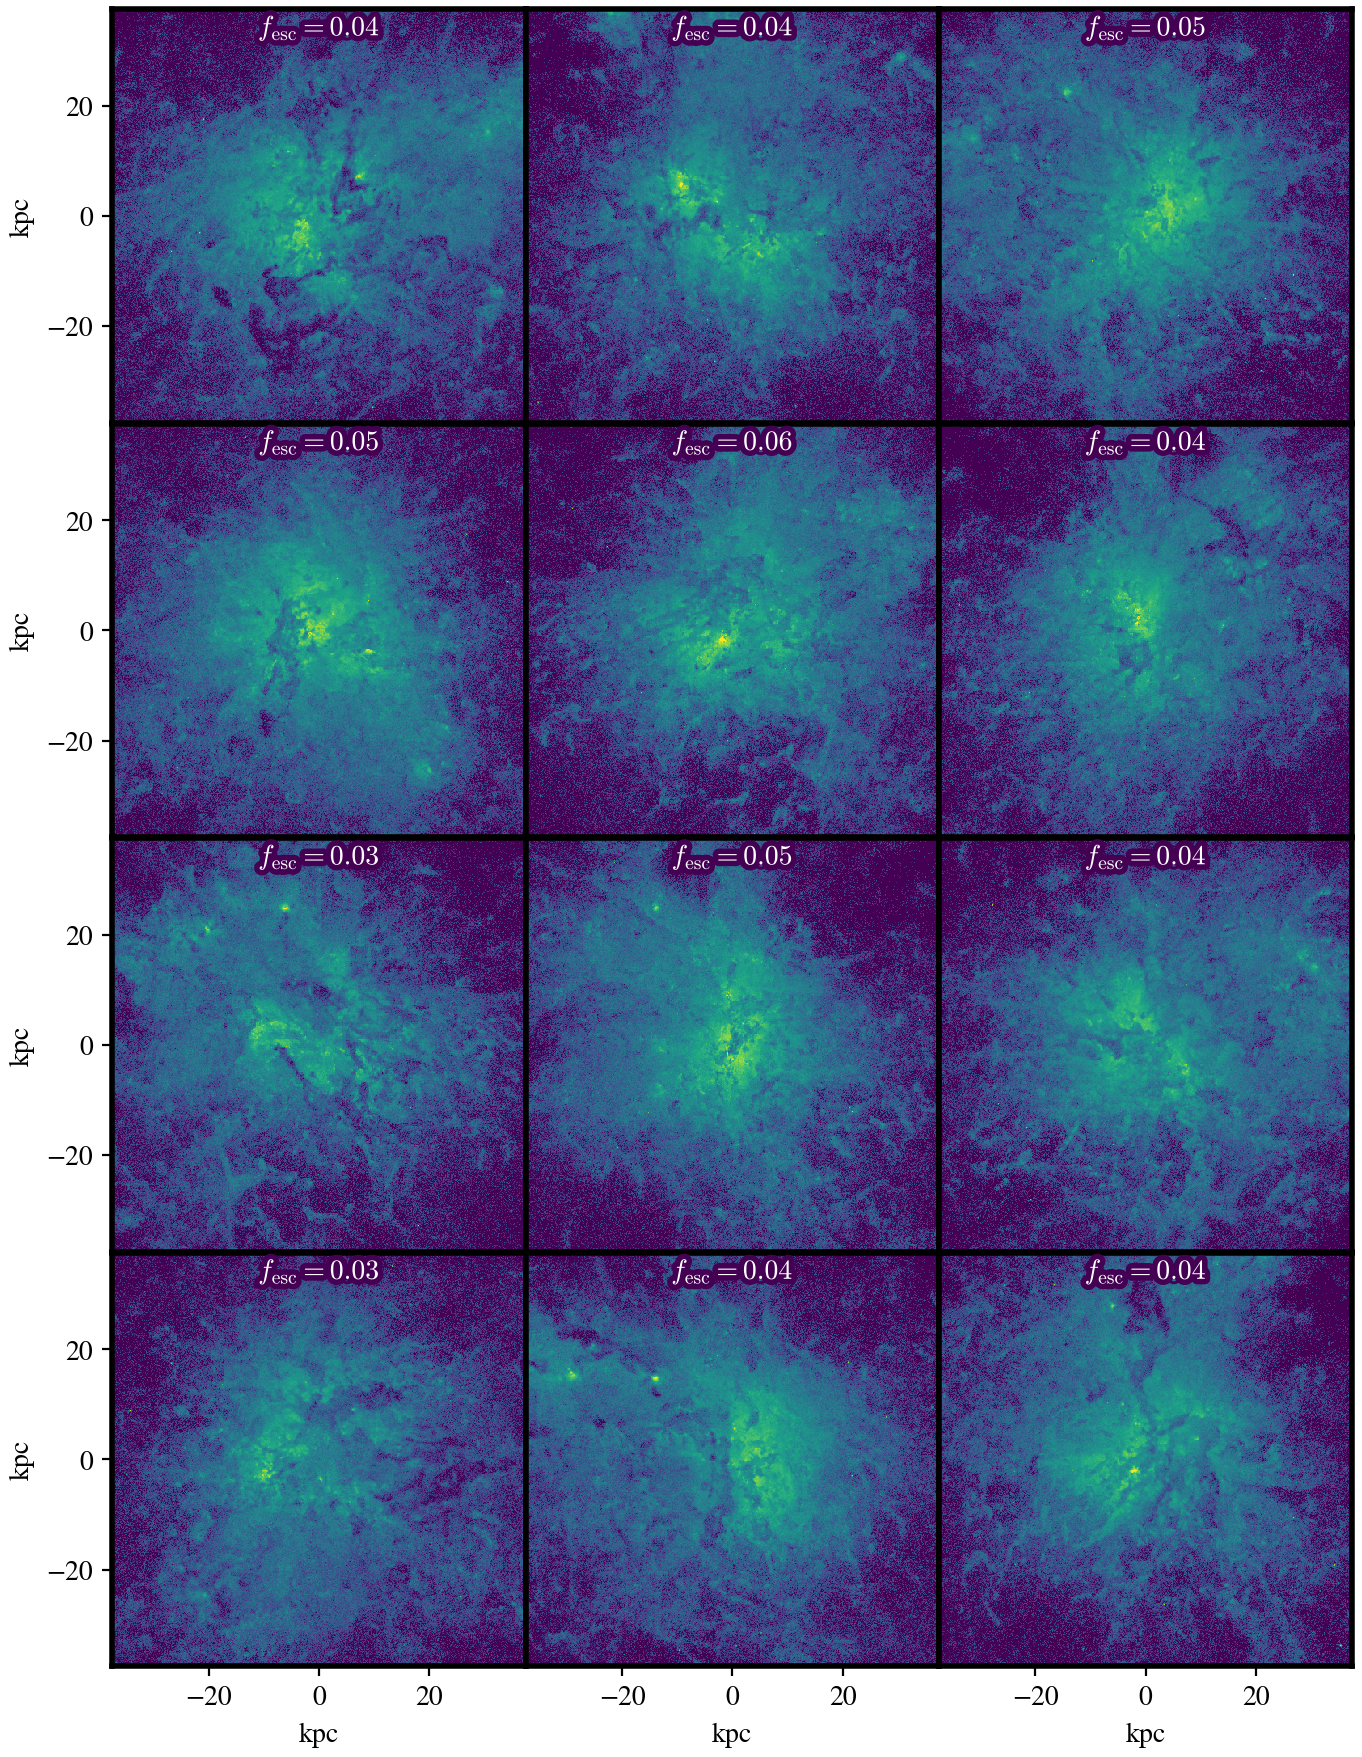
\includegraphics[width=\textwidth,height=\textheight,keepaspectratio]{figures/many_los.png}
    \caption{
        A single snapshot from halo A8 at redshift $z=2.4$, seen from 12 equally spaced lines of sight.
        The surface brightness is scaled between $2\times10^{-15}$ and $10^{-19}$ $\rm{erg}\ \rm{s}^{-1}\ \rm{cm}^{-2}\ \rm{arcsec}^{-2}$, to enhance the line-of-sight contrast.
        Compare to Figure~\ref{fig:many_los}, which includes our model for AGN.
    }
    \label{fig:many_los}
\end{figure}

\begin{figure}
    \centering
    \includegraphics[width=\textwidth,height=\textheight,keepaspectratio]{figures/agn_many_los.png}
    \caption{
        A single snapshot from halo A8 at redshift $z=2.4$, seen from 12 equally spaced lines of sight.
        We have selected this snapshot because it has the greatest variance in escape fraction with line of sight.
        The surface brightness is scaled between $2\times10^{-15}$ and $10^{-19}$ $\rm{erg}\ \rm{s}^{-1}\ \rm{cm}^{-2}\ \rm{arcsec}^{-2}$, to enhance the line-of-sight contrast.
        Compare to Figure~\ref{fig:many_los}, which does not include our model for AGN.
    }
    \label{fig:agn_many_los}
\end{figure}


\section{The impact of AGN on the spatial extent and concentration of Ly\texorpdfstring{$\alpha$}{a} in blobs}

As in the overall Ly$\alpha$ luminosity, the AGN can also impact the spatial extent of Ly$\alpha$ emission in massive halos.
This takes two forms: (1) the total area enclosed within a surface brightness contour and (2) the concentration of Ly$\alpha$ light in the system.
We explore these in turn.

Previously, in Figure~\ref{fig:area_plot}, we examined the size of our model LABs as a function of observation sensitivity (solid lines) for example snapshots that did not have AGN on.
Now in Figure~\ref{fig:agn_area_plot} we include dashed lines for example snapshots with the AGN in our model.

We see an enhancement of blob size at high surface brightness cutoffs, which indicates that there are regions that have been substantially enhanced in brightness, but at the same time we see a decrease in blob size at much lower cutoffs.
We interpret this effect as a complex interaction of the gas ionization state with escape pathways.
As gas becomes more ionized it provides a pathway along which Ly$\alpha$ is likely to escape; it is these pathways that produce the small region(s) of very intense surface brightness.
However, the presence of a low-opacity pathway out of the blob decreases the probability that a photon will be scattered out into the extended blob structure before it escapes.

The presence of these small pathways out of blob may be useful to detect the presence of AGN in a blob.
We quantify the concentration of light by computing the Gini coefficient $G$ of a surface brightness image which is composed of $n$ pixels $p_{0}..p_{n}$ of each blob, which we present in Figure~\ref{fig:skewness}.
\begin{equation}
    \label{eq:gini}
    G = \frac{2\sum_{i=1}^{n}i p_{i}}{n\sum_{i=1}^{n}p_{i}} - \frac{n+1}{n}
\end{equation}
The primary signature of the AGN's effect is to cause the luminosity to be concentrated in a much smaller area.
While this may seem contradictory to the increase in total luminosity and area enclosed, note that this is a {\it relative} concentration.
That is, while the diffuse emission is still significant, the central emission in the ionized bubble surrounding the AGN dominates when compared to this diffuse halo emission such that the overall concentration decreases dramatically for the AGN-on model.
This metric becomes more effective for identifying AGN with higher-resolution observations (Figure~\ref{fig:MUSE}) since the bright patches of our surface brightness images are significantly smaller than the spatial resolution of current telescopes, but current technologies should be sufficient.

\begin{figure}
    \centering
    \includegraphics[width=\textwidth,keepaspectratio]{figures/skew_distribution.pdf}
    \caption{
        In our surface brightness images with AGN, the escaping luminosity is much more spatially concentrated.
        We quantify this trend by computing the Gini coefficient for a number of halos with and without AGN, after convolving to the resolution of MUSE.
        By selecting a Gini coefficient threshold around 0.93, one could reliably distinguish between blobs that contain and do not contain AGN.
    }
    \label{fig:skewness}
\end{figure}


\section{Impact of AGN model}

In the preceeding sections, we have referred to a particular AGN model wherin we derive the ionizing luminosity of each black hole particle from their masses assuming an Eddington accretion rate with efficiency of $0.1$ and a \citet*{Hopkins2007} template.
All these assumptions can be adjusted individually; we could use a different AGN template (such as \citet{Nenkova2008}), we could derive luminosities from the black hole particle accretion rates instead of their masses, we could assume a different efficiency, and we could ignore the black hole particles provided entirely, substituting masses compute from the relation derived by \citet{Magorrian1998}.
All of these changes would amount only to altering the luminosity of the super-massive star particles we feed into our ionization state calculation, so we pursue all of these by investigating whether the luminosity of a halo is related to the efficiency parameter, which we vary over the range $[0.01, 1.0]$.
This gives us an order of magnitude variation in either direction from our best-guess model and so should encompass any relevant trends in this parameter; we plot the results of this experiment in Figure~\ref{fig:eddington_grid}.

\begin{figure}
    \centering
    \includegraphics[width=\textwidth,keepaspectratio]{figures/skew_distribution.pdf}
    \caption{
        We vary the black hole efficiency in our AGN model by an order of magnitude; from our best-guess value of $0.1$ down to $0.01$ and up to $1.0$.
        There is no simple correlation between the AGN luminosity in our model and Ly$\alpha$ luminosity.
    }
    \label{fig:eddington_grid}
\end{figure}

As with every other aspect of this work, the relation we find defies simple explanation.
From a naive perspective, one would expect the luminosity of the blob to increase, possibly linearly, with the luminosity of the AGN but it does not.
This scenario is qualitatively similar to the trend we discussed in \S~\ref{sec:agn_blob_luminosity}, but in this case the covering fraction argument does not hold, and thus we left with two possibilities here.
The first is that the progressive ionization is very inhomogenous, which causes what looks like random changes in the blob's luminosity as smaller-scale RT effects dominate.
The luminosity may increase when a new large-scale pathway is opened out of the blob, or it may decrease if the geometry shifts into a configuration which more efficiently traps Ly$\alpha$.
The alternative explanation is that this behavior is numerical, not physical in nature.
We can confirm that the luminosity values at any particular $f_{\rm{Eddington}}$ are stable from run to run which should rule out Monte-Carlo noise, but we do not fully understand the convergence of the ionization state calculation, so it is hard to predict if whatever unconvergence is left coupled with how self-inconsistent this system has been made could be responsible for this fluctuation of Ly$\alpha$ luminosity.

\chapter{Numerical Experiments}
\label{sec:experiments}

\section{Impact of the UV Background}
The original objective of this project included a study of the dominant physical sources of Ly$\alpha$ emission, which we assumed would be stars, cooling from accreting gas, and the cosmological UV background.
As as apparent from the aforementioned text in this dissertation, the structure of the project has shifted since then, most notably to consider the underlying physical mechanisms (recombinations vs collisions) as opposed to the astrophysical origins (stars vs UV background vs accretion).
Primarily, this is because the impact of stars or accretion is manyfold and therefore we cannot simply turn them off or adjust their intensity and maintain much self-consistency in the simulation.

That is, ideally we would ask some question along the lines of "What is the impact of the UV background on the formation of Ly$\alpha$ blobs?" and could answer this question by turning off the UV background and observing an impact on the Ly$\alpha$ luminosity and escape fraction.
However, we cannot address this question in such a direct manner because the impact of this phenomenon is imprinted on the temperature of the gas during the hydrodynamical simulations we rely on as inputs.

Instead, in this section we present an experiment wherein we increase the intensity of our post-processing non-heating treatment of the UV background to gain some intuition for the impact of this phenomenon on the formation of Ly$\alpha$ blobs.
We increase the intensity of the UV background from a redshift-dependent value derived from \citet{Faucher-Giguere2009} of $1.2\times10^{-22}\ erg\ cm^{-2}\ s^{-1}\ Hz^{-1}$ up to a non-physical increase of 5 orders of magnitude (Figures~\ref{fig:big_uv_000} and \ref{fig:big_uv_005}), and find that this provides only a small enhancement to the luminosity of the blob and if anything makes it less like a blob by decreasing its spatial extent.
Our interpretation of this slight increase in luminosity and decrease in spatial extent is that the primary effect of the UV background increase is to ionize extended neutral gas which resonantly scatters the Ly$\alpha$ to greater spatial extents, permitting Ly$\alpha$ to escape the blob with less scattering.
Therefore we rule out the UV background as a driver of LAB formation and declare enhancements in the UV background uninteresting, since we increase it to a nonphysical value and still only see a marginal effect (recall that we cannot really remove the UV background because the heating it causes is accounted for in the gas temperature).


\begin{figure*}
    \centering
    \includegraphics[width=\textwidth,keepaspectratio]{figures/big_uvb_000.pdf}
    \caption{
        A surface brightness image of a sample halo, with the UV background intensity from \citet{Faucher-Giguere2009}.
    }
  \label{fig:big_uv_000}
\end{figure*}

\begin{figure*}
    \centering
    \includegraphics[width=\textwidth,keepaspectratio]{figures/big_uvb_005.pdf}
    \caption{
        A surface brightness image of a sample halo, with a UV background intensity set to $10^{5}$ times that in Figure~\ref{fig:big_uv_000}.
    }
  \label{fig:big_uv_005}
\end{figure*}



\section{MCRT Convergence}
Sometimes radiative transfer work is referred to as simulations but we try to avoid that term in this section.
Instead, we find it much better to call all our RT codebases solvers instead of simulations because they do not involve a time domain, and because each execution of the program proceeds through a numerical process which proceeds towards a consistent result through a different pathway.
Ideally, we'd like to know if our radiative transfer is converged.
But answering that question is very complex as we will discuss later, so in this section we present some preliminary work on a metric for the convergence of surface brightness images.

Ideally, we should have an on-the-fly metric that measures how uncertain a particular value in our radiative transfer calculation is.
Since some of our work is centered around surface brightness images, a reasonable first step is to establish a metric for determining if any given pixel is converged.
To approach this, we insert a notional error map into {\sc colt}, where the uncertainty $\sigma$ of a pixel in the map due to $i$ next event estimations $e$ is
\begin{equation}
    \sigma \propto \frac{\sqrt{\Sigma_{i} e_{i}^{2}}}{\Sigma_{i} e_{i}}
    \label{eq:sb_uncertainty}
\end{equation}
This metric is essentially the relative variance within the pixel, and from a naive perspective is an effective way to track the uncertainty.
We plot this metric for one of our surface brightness images in Figure~\ref{fig:on_the_fly}.
To check how accurate this is, we run {\sc colt} 300 times with the same inputs and plot the per-pixel variance in Figure~\ref{fig:run_to_run}, which should match with Figure~\ref{fig:on_the_fly}.
As we can see, this simple on-the-fly uncertainty estimate vastly underestimates the variation in a pixel between executions of the code.

We believe this simplistic metric is wrong because each next event estimation contribution to a pixel is not a measurement of the luminosity of that pixel.
How one could correctly derive a convergence metric in the face of this is beyond the scope of this paper because it requires statistics expertise we do not posess.
Instead, our purpose here is to present these results because they cost many CPU-hours and we have verified that using a naive approach to on-the-fly assessment of MCRT convergence results in an incorrect metric.
Future work on this should instead follow methodologies used in Markov Chain Monte-Carlo (MCMC) techniques, and in particular we suggest the Gelman-Rubin diagnostic may be a much better indicator of convergence (Aaron Smith, private communication).

\begin{figure*}
    \centering
    \includegraphics[width=\textwidth,keepaspectratio]{figures/on_the_fly.pdf}
    \caption{
        For a sample halo, we plot the relative uncertainty reported by Eq~\ref{eq:sb_uncertainty}.
    }
  \label{fig:on_the_fly}
\end{figure*}

\begin{figure*}
    \centering
    \includegraphics[width=\textwidth,keepaspectratio]{figures/run_to_run.pdf}
    \caption{
        For a sample halo, we plot the relative 1-$\sigma$ uncertainty computed across 300 runs of {\sc colt}.
        Note that this uncertainty is much greater than what is estimated in Figure~\ref{fig:on_the_fly}.
    }
  \label{fig:run_to_run}
\end{figure*}


\section{Ionization State Extremes}
\label{sec:ionization_extremes}
In this work we have made somewhat of a big deal out of the ionization state of the gas because it is related to Ly$\alpha$ luminosity, escape fraction, and also determines which of the two physical mechanisms (recombination and collisional excitation) dominates.
For most of our work we endeavor to recreate the physical conditions that exist in nature, but of course we can write a little bit of code and adjust the physical conditions in a simulation to whatever we desire.

In this section we use this ability to get some handle on how bright a blob could be due to recombinations or collisional excitations if the ionization state of the gas were tuned such that those mechanisms were as dominant as possible.
In the case of recombinations, we consider a scenario where all gas in the simulation is fully ionized.
This is nonphysical because there is dense cool gas in the simulation which would rapidly recombine then stay recombined if this were the case, but of course we need not let that stop us.
We present the results of this experiment in Figure~\ref{fig:rogues_fully_ionized}.
These images can be compared to Figure~\ref{fig:rogues4}, with the caution that a number of pixels that have increased in brightness are clipped in these surface brightness images produced with the altered ionization state.
We prefer this visualization to one where we have altered the scaling because it is easier to compare to the physically motivated model.
In these images, the blob appears to have shrunk even though we have altered the ionization state of the gas such that overall it enhances the luminosity of the blob.
This size decrease should not be too surprising; by ionizing the gas we have removed resonant scattering from the model so what is left is nearly a projection of Ly$\alpha$ surface luminosity (but with Monte-Carlo noise and some dust scattering).
Additionally, the luminosity in this case is enhanced by about 2 orders of magnitude; these halos have a luminosity of about $5\times10^{45}\ \rm{erg}\ \rm{s}^{-1}$

\begin{figure*}
    \centering
    \includegraphics[width=\textwidth,height=0.9\textheight,keepaspectratio]{figures/rogues_fully_ionized.png}
    \caption{
        Ly$\alpha$ surface brightness images of halo A4 from $z=4.5$ (top-left) to $z=2.0$ (bottom-right).
        All images are 75$\times$75 physical kpc across, and are scaled from $2\times10^{-19}-10^{-16}\ \rm{erg}\ \rm{s}^{-1}\ \rm{cm}^{-2}\ \rm{arcsec}^{-2}$.
    }
  \label{fig:rogues_fully_ionized}
\end{figure*}


We also conduct another experiment in which we set the ionization state of all the gas to $0.5$, to maximize the emission due to collisional excitation.
The results of this experiment are presented in Figure~\ref{fig:rogues_half_ionized}.
In this experiment we must rescaled the surface brightness images to accommodate the increased luminosity of the gas, otherwise the entire surface brightness images would be clipped.
Additionally, the luminosity in this case is enhanced by about 3 orders of magnitude; these halos have a luminosity of about $2\times10^{46}\ \rm{erg}\ \rm{s}^{-1}$.
Naively one might expect these simulations to have a much lower escape fraction since we have taken a large amount of halo gas which was previously fully ionized and put in an ionization state where it is more likely to keep Ly$\alpha$ trapped.
This is not the case; overall we see escape fractions which are approximately the same as the physically motivated case.
Most likely, this is driven by the increased emission in the hot gas which can easily escape the simulation compensating for the increased absorption of gas emitted in the more dense regions of the simulation.

\begin{figure*}
    \centering
    \includegraphics[width=\textwidth,height=0.9\textheight,keepaspectratio]{figures/rogues_half_ionized.png}
    \caption{
        Ly$\alpha$ surface brightness images of halo A4 from $z=4.5$ (top-left) to $z=2.0$ (bottom-right), where we have artificially set the ionization state to $0.5$.
        All images are 75$\times$75 physical kpc across, and are scaled from $1\times10^{-13}-10^{-17}\ \rm{erg}\ \rm{s}^{-1}\ \rm{cm}^{-2}\ \rm{arcsec}^{-2}$.
    }
  \label{fig:rogues_half_ionized}
\end{figure*}



\chapter{Conclusions and Future Directions}
\label{sec:discussion}

\section{Conclusions}
\label{sec:conclusions}


\section{The Case for Rad Hydro}

The most uncertain part of this project is the ionization state and temperature of the gas, and most unfortunately that is the most out-of-scope improvement that could be made to this work.
The core problem is that the hydrodynamic simulations this work is based on do not include an accurate accounting for the effect of the UV background and the ionization of gas due to stars.
There are approximations for both of these, but they are very coarse and not self-consistent.
Specifically, the approxiamation for the cosmological UV background assumes that there is an ever-present UV field in the simulation, and thus ignores that the self-shielding effect of any neutral gas in the simulation against the cosmological UV background.
The approximation for stars is that a star will ionize some mass of gas near it, which while it does not ignore self-shielding entirely does tend to ignore radiative transfer effects that may cause highly asymmetric structure in the ionization state of the gas.
If there is one lesson from this work it is that radiative transfer rapidly becomes complex, so we are very wary of such an approximation.
Unfortunately fixing these problems properly requires an on-the-fly treatment of the feedback loop between the heating of gas, resultant collisional ionization, radiative transfer of ionizing energy, radiative ionization, then re-calculation of the radiative transfer due to updated opacity of the gas.
This is not computationally cheap, but may be critical for future more accurate Ly$\alpha$ studies.

To be clear, the work we have done here in post-processing is not a panacea; this \emph{must} be done on-the-fly because all computations done in post-processing will not be self-consistent.
In this work, we try to compute a more accurate ionization state at a timestep $t$ based on the physical conditions at $t$, but the ionization state will alter the evolution of the simulation.
Therefore, the physical conditions we base our ionization state at time $t$ upon are incorrect, and we actually needed to do this more accurate calculation at timestep $t-1$ and so on.

\section{Ly$\alpha$ flow and radiation pressure}

\section{Software Future Directions}

It's generally accepted that most code in the world is vastly slower than it could be, even if it's written by experts in a language like C++.
But software in astronomy is somewhat of an extreme case, for a number of reasons.
With the growth of data in the field (and especially in this project) a number of strategies that were technically sub-optimal but not a serious issue are heading towards that.
In this project there are two specific examples: Numerical tables stored in text files, and eager initialization of large data structures.
Storing data in a text format is a very attractive solution for data interchange; unlike all other formats if documentation is lost entirely at least the data itself can be recovered (if not the semantics thereof).
But text files are rather slow to read, and the common tools for reading and writing them are embarrassingly slow. To be clear, we are referring to \lstinline{fprintf} and \lstinline{fscanf} and in the Python world, \lstinline{numpy.savetxt} and \lstinline{numpy.loadtxt}.
A disappointing (but not large in an absolute sense) amount of time in this project was spent waiting for text files to save or load.
There are partial solutions to this problem; reading and writing of text formats can be made much faster.
For example \href{https://github.com/saethlin/loadtxt}[loadtxt] can load text files much faster than tools in \lstinline{numpy}, and a similar approach could be taken using Ulf Adams's ryu algorithm for saving text files (though as with code, reading is the more common operation).

The HDF5 format is a much better solution to rapidly reading data from files.
It's fast enough, supports transparent compression, and allows adding metadata to files and datasets within a file.
This could even be used to associate units with data.

\subsection{Octrees}

Much of this work involves octrees, which are a rather common data structure in simulations in general.
While we use them as an adaptive grid, they're often also used as a way to look up nearest neighbors in a particle simulation.
Navigating an octree does not dominate the runtime of \textsc{colt}, but it does dominate the runtime of \textsc{lycrt}, and it can dominate the runtime of some other codes like \textsc{gizmo} when additional self-gravitating particles are added.
For this reason, one might naively expect that there exists a highly-polished implementation of an octree that is used ubiquitously, or at least that the data structure is well-studied enough that the most optimal implementation strategies are well-established.
Unfortunately, this does not seem to be the case.
We include below, the approximate definition of the octant structure used in \textsc{lycrt} (it has been cleaned up a bit).
\begin{lstlisting}
struct Cell {
    double width;
    double min_x[3];

    long parent_ID;
    long sub_cell_check;
    long sub_cell_IDs[8];

    LOCALVAL *U;
    int HAS_U_ALLOCATED;
};
\end{lstlisting}
For comparison, here is a similarly cleaned-up version of the octant structure used in the public \textsc{gizmo} codebase.
\begin{lstlisting}
struct Node {
  MyFloat center[3];
  MyFloat len;

  union {
    int suns[8];
    struct {
      MyFloat s[3];
      MyFloat mass;
      unsigned int bitflags;
      int sibling;
      int nextnode;
      int father;
    } d;
  } u;
};
\end{lstlisting}

These implementations have something in common; 


\end{document}
